\documentclass{ou-report}
%% \citestyle{agu}

\usepackage{booktabs}

\newcommand{\HJ}[1]{{\color{red} HJ: #1}}
\newcommand{\todo}[1]{{\color{red} TODO: #1}}
\newcommand{\vraag}[1]{{\color{teal} {\textbf{VRAGEN AAN HUGO: }}#1}}
\newcommand{\outline}[1]{{\color{blue} #1}}
\newcommand{\old}[1]{{\color{gray} #1}}

\newcommand{\doi}{{DOI}}
\newcommand{\lncs}{LNCS}
\newcommand{\dblp}{DBLP}
\newcommand{\api}{API}
\newcommand{\orcid}{ORCID}

\usepackage{float,wrapfig}
\usepackage{tikz}
\usepackage[shortlabels]{enumitem}
\usepackage[normalem]{ulem}
\usepackage{multicol}

\usetikzlibrary{positioning}
\usepackage{graphicx}
\usepackage{centernot}
\usepackage{lscape}


%% Die gekke Hugo wil paragrafen met punten... tsk.
\usepackage{xparse}
\usepackage{amsthm}
\makeatletter
\let\latexparagraph\paragraph
\RenewDocumentCommand{\paragraph}{som}{%
  \IfBooleanTF{#1}
    {\latexparagraph*{#3}}
    {\IfNoValueTF{#2}
       {\latexparagraph{\maybe@addperiod{#3}}}
       {\latexparagraph[#2]{\maybe@addperiod{#3}}}%
  }%
}
\newcommand{\maybe@addperiod}[1]{%
  #1\@addpunct{.}%
}
\makeatother

% Settings for code fragments
\lstset{
  basicstyle=\fontsize{9}{13}\selectfont\ttfamily,
  showstringspaces=false
}

% Dit template is gemaakt door P.J. Molijn in het kader van zijn afstuderen aan de OU in 2014.
% Waarvoor hartelijk dank.
% Minieme maar belangrijke wijzigingen zijn aangebracht door E.M. van Doorn
% Het template is versimpeld door Sylvia Stuurman, 2019.


%\hypersetup{
%pdfsubject={Master Thesis <Titel>, <author>},
%pdfkeywords={keyword1, keyword2}
%}


\setlist{noitemsep}

\begin{document}
\pagestyle{plain}
%% \title{Applying outlier detection on the scientific publication process to support fraud detection}
\title{Acquisition and integration of public data to improve detection of scientific fraud}
%% \title{Improving detection of scientific fraud by enriching the publication model with public data}
\author{Ewoud Westerbaan}
%Title of the thesis
%\title[Subtitle]{Title}
%\author{author}
%\affiliation{
%\begin{tabular}{ll}
%Student: & studentnumber \\
%Date:    & DD/MM/YYY \\
%\end{tabular}
%}
%
%%\coverimage{cover/cover.jpg}
%%            ===============
%\makecover[frontboxwidth=4.6in]
\begin{titlepage}

\begin{center}

%% Insert the OU logo at the bottom of the page.
\begin{tikzpicture}[remember picture,overlay]
    \node at (current page.south)[anchor=south,inner sep=0pt]{
        
\includegraphics[scale=0.7]{cover/logo}
    };
\end{tikzpicture}

%% Extra whitespace at the top.
\vspace*{2\bigskipamount}

%% Print the title in specific color.
{\makeatletter
%\titlestyle\color{ou-cyan}\Huge\@title
\titlestyle\color{red}\Huge\@title\par
\makeatother}

%% Print the optional subtitle in black.
{\makeatletter
\ifx\@subtitle\undefined\else
    \bigskip
    \titlefont\titleshape\LARGE\@subtitle
\fi
\makeatother}

\bigskip
\bigskip

by
%door

\bigskip
\bigskip

%% Print the name of the author.
{\makeatletter
\titlefont\Large\bfseries\@author
\makeatother}

\vfill

in partial fulfillment of the requirements for the degree of
%in overeenstemming met de vereisten voor het verkrijgen van de graad van

\bigskip
\bigskip

{\bfseries Master of Science}

in Software Engineering

\bigskip
\bigskip

at the Open University, faculty of Management, Science and Technology \\
Master Software Engineering
%aan de Open Universiteit Nederland,

to be defended publicly on Day Month DD, YYYY at HH:00 PM.
%in het openbaar te verdedigen op dinsdag 9 september om 15:00 uur.

\vfill

\begin{tabular}{lll}
%% Add additional information here, per faculty requirements, e.g
    Student number: & 852069942 \\
    Course code: & IMA0002\\
    Thesis committee:
        & titles and name of the chairman (chairman), & Open University \\
        & titles and name of the supervisor (supervisor), & Open University
\end{tabular}

%% Only include the following lines if confidentiality is applicable.
\bigskip


\bigskip

\end{center}

\end{titlepage} 


%% Use Roman numerals for the page numbers of the title pages and table of
%% contents.
\pagenumbering{roman}
%% Include an optional title page.

\frontmatter 


\let\cleardoublepage\clearpage

% Optional Dedication, Acknowledgement
%\input{dedication}

%\input{acknowledgement}
\tableofcontents

%Optional: list of figures, list of tables
%\listoffigures

%\listoftables

%% Include an optional summary page.
%\input{Summary/summary}
%\input{Summary/samenvatting}

\mainmatter
\pagenumbering{arabic}


\newcommand{\mi}[1]{\ensuremath{\mathit{#1}}}
\newcommand{\authors}{\mi{authors}}
\newcommand{\cites}{\mi{cites}}
\newcommand{\receives}{\mi{receives}}
\newcommand{\reviews}{\mi{reviews}}
\newcommand{\accepts}{\mi{accepts}}
\newcommand{\rejects}{\mi{rejects}}
\newcommand{\editorinchief}{\mi{EiC}}
\newcommand{\associateeditor}{\mi{AE}}
\newcommand{\Humans}{\mi{People}}
\newcommand{\Reviewers}{\mi{Reviewers}}
\newcommand{\Editors}{\mi{Editors}}


% ==============================================================================
\chapter*{Abstract}
% ==============================================================================

\paragraph{Situation}
The output of scientists is assessed by metrics like number of publications 
and citations. To turn these metrics to their benefit, various forms of fraud
are being conducted.
For fraud in publications, like plagiarism, various detection methods are in
place. However, for post-publication fraud (fraud conducted after the actual
production of an article) these detection methods are not structural in place
and detection requires a lot of human effort.
Improvement in detecting these types of fraud is to direct this human effort to
the most egregious cases. However, generic approaches to detect these cases 
have failed because:
\begin{itemize}
    \item Detection is applied on the whole population: a person can be outlier
        within a subgroup (e.g. editor targets its own journal, but other editors do not), 
        but not within the whole population (other authors also target that journal);
    \item Public datasets these research are based upon, are too limited.
\end{itemize}

\paragraph{Research}
In this research we investigate the added value of enriching existing publicly
datasets with not yet integrated publicly available data for directing manual
effort for fraud detection in the publication process. As validation we apply 
a group based outlier detection.

\paragraph{Main contributions}
Our main contributions are:
\begin{enumerate}
    \item Improved set-theoretic publication datamodel which can be used to 
        reason about the publication model. Sources to load this model are 
        discussed.
    \item Acquisition methods to gather the necessary data to improve existing 
        publicly available datasets. These enriched datasets can be used for
        fraud detection.
    \item Case studies where we define sets gathered from public and additional
        acquired data. On these sets we apply a limited analysis to identify 
        outliers. This is the proof our approach is actually working.
    \item Recommendations to the research community which improves the detection of 
        fraud on the publication process. 
\end{enumerate}

\paragraph{Key points}
The results of this research are:
\begin{itemize}
    \item For this study, it is not feasible to create one integrated dataset
        out of multiple publicly available datasets;
    \item Enriching standard datasets (datasets prepared for publication process
        analysis) is made more difficult because of diffusion coupled with lack
        of structure of data;
    \item Applying group based approach on enriched data yields useable results.
\end{itemize}


% ==============================================================================
\chapter{Introduction}
% ==============================================================================
Incentives for scientists rely on quantitative measures of science, such as 
number of publications, number of citations and amount of grants received. 
However, as the aphorism known as Goodhart's Law states: ``When a measure 
becomes a target, it ceases to be a good measure''~\cite{strathern_1997}. That 
is the case here as well: these metrics not only incentivise scientific 
excellence by doing research and publishing the results; they also invite, 
maybe even more rewarding, dishonest approaches to achieve high rankings 
-- gaming of these metrics, or, more simple, fraud in scientific publishing. 

An interesting example where Goodhart's Law could play a role is the following
case: In 2010, Italy started using the number of citations as input for academic
promotion. Seeber et al.~\cite{SEEBER2019478} investigated whether this
increased the number of  self-citation. In Figure~\ref{fig:seeber}, Seeber et
al.~show the number of self-citations per year (the 2009 spike is not
discussed).
While the intuitive argument is clear, whether the data backs this up is subject
to interpretation. It is clear from the graphs that the variance between various
groups of academics is greater than the impact of the new rule. Data on the
whole of Italian academia would therefore probably only show a slight increase.
In reality, in certain subfields, the average number of self-citations would
have more than doubled.

\begin{figure}[H]
\centering
\includegraphics[width=16cm]{images/introduction/seeber_annotated.PNG}
\caption{Evolution of self-citations per article (adapted from~\cite{SEEBER2019478}).
    The red line indicates the moment citation-rates became input for promotion.}
\label{fig:seeber}
\end{figure}

Other examples of fraud include plagiarism, manipulation  of images
(e.g., of cell extracts in life science publications), manipulation of research
data, fabrication of research data. In addition, there may be as-of-yet unknown
forms of fraud.

Various prevention and detection measures are in place. In absence of these 
deterrents, the scientific process would be vulnerable to dishonest behaviour. 
These existing deterrents are typically focused on specific forms of dishonest 
behaviour. Examples of these existing measures are Ithenticate to detect 
plagiarism, or ORI's Forensic
Droplets\footnote{\url{https://ori.hhs.gov/droplets}} 
to detect manipulated images. The practice of preregistration ensures scientific
studies are conducted as planned, and helps to prevent data manipulation such as
p-hacking\footnote{P-hacking is manipulation of the data so the research becomes
statistically important.}. Another measure is applying statistical evaluation to
uncover manipulation of research data~\cite{HGWA2019}. 

Despite these deterrents, some forms of dishonest behaviour still slip through.
Examples of such behaviour are:
self-nominating as reviewer (e.g. Moon), forced citation (authors are being
forced to cite work), forced co-author-ship (forced to name a person as
co-author).
Such behaviours use dishonest tricks outside the detective capabilities of
current detection methods and therefore escape initial scrutiny. We know of
such cases typically through whistle blowers and manual investigation. 
This illustrates that a problem still exists, yet the scale of the
problem remains unknown.

In particular, one obstacle to prevent this problem is the huge (and growing) 
number of scientific 
publications and scientific authors. For example, the DBLP website, which 
records most publications in computer science, currently lists more than 
2.5~million authors -- a number that cannot be manually investigated. 
Another obstacle is the cost involved to investigate the possible scientific 
misconduct~\cite{MHWT2010}.
Hence, a more generic approach to detect fraud is needed. 


% \todo{
% \begin{itemize}
%     \item dus: Generieke vorm van detectie gewenst
%     \item dat kan dus niet afhangen van een specifieke aanval
%     \item dat moet dus gebaseerd zijn op een holistische view van het 
%         publicatieproces (kerngetallen bijvoorbeeld)
%         -- en weten wat daar de norm is.
%     \item Dus beschouwen we in de volgende secties het publicatieprocess in meer 
%         detail.
% \end{itemize}
% }
% ==============================================================================

In this project, we aim to take a step in this generic approach by not 
focusing on the method of fraud applied, but on the 
\emph{effect of scientific fraud}, by taking a holistic view of the publication 
process. We tend to do this in two steps:
\begin{enumerate}
\item Provide a concise underlaying integrated datamodel;
\item Identify outliers within groups sharing characteristics.
\end{enumerate}
% We tend to do this in two 
% steps:
% \begin{enumerate}
%     \item The first step is to identify groups of people sharing a 
%         charateristic (e.g. same role).
%     \item The second step is to identify outliers within this group based on
%         other characteristics (e.g. number of publications).
% \end{enumerate}
% Other examples are given in 
% Section~\ref{interesting_cases}.

The underlying assumption this approach is based upon, is that the various types 
of scientific fraud all 
share a common characteristic: their goal is the same, that is, their goal 
is to improve a researcher's or publication's quantitative measures of 
science. This elevates them above their peers -- which on the one hand 
brings recognition and accolades, but on the other, makes them stand out. In 
short, the underlying assumption is that fraudsters aim to become outliers 
(in terms of quantitative measures of science).

To clarify this with an example: An editor of a journal publishes in his 
own journal to boost his publication metrics. This may be fraudulent behaviour. 
If other editors of this same journal do not publish (or publish much less), 
this editor of interest is considered an outlier, because of the discrepancy 
with his group of peers. 
We immediately caution that the implication representing our assumption
(\emph{fraud} $\implies$ \emph{outlier})
does not hold in reverse. That is: such outliers need not be fraudsters: 
(\emph{outlier} $\centernot\implies$ \emph{fraud}). 
However, identifying outliers may reduce the pool of authors to be investigated
by several orders of magnitude. Thus, while not perfect, outlier classification
should make manual investigation of cases where fraud would have had significant
effect possible.

The goal of this project is to take a first step to make this a possibility.
Concretely, our research objective is to integrate multiple data sources to
enable the possibility of performing a group based outlier detection.
% ------------------------------------------------------------------------------
The focus of this study is on the computer science 
discipline. For other disciplines the approach of this research probably needs
to be tuned specifically. 
For example: the average number of co-authors per article change between
research areas\footnote{\url{https://www.natureindex.com/news-blog/paper-authorship-goes-hyper}}.

% ==============================================================================
\ \\
During this research we will contribute the following items:
\begin{itemize}
    \item \emph{Improved set-theoretic publication datamodel} which can be used
        to reason about the publication model. Sources to load this model are 
        discussed.
    \item \emph{Acquisition methods} to gather the necessary data to improve
        existing publicly available datasets. These enriched datasets can be
        used for fraud detection.
    \item \emph{Case studies} where we define sets gathered from public and
        additional data. On these sets we apply a limited analysis to identify
        outliers. This is the proof our approach is really working.
    \item \emph{Recommendations} to the community which increases the detection
        of fraud on the publication process. 
\end{itemize}


This thesis will continue with a domain analysis of the publication process in
Chapter~\ref{chp:domainanalysis}. After this background chapter, other 
related work is discussed in Chapter~\ref{chp:related_work}. The used
methodology is described in Chapter~\ref{chp:methodology}. 
From here on we will
answer the research questions which starts with the datamodel and - acquisition
in Chapter~\ref{chp:data}, a generic implementation in 
Chapter~\ref{chp:generic_implementation} and follows with three case studies in 
Chapters~\ref{chp:case1}, \ref{chp:case2} and \ref{chp:case3}. 
We end this thesis with the conclusions in Chapter~\ref{chp:conclusions} with
recommendations in Section~\ref{sec:recommendations} and discussion in
Section~\ref{sec:discussion}.

% In Chapter~\ref{chp:graph_based_approach} we perform an initial exploration of 
% the generic applicability of a graph based approach for fraud detection.



% ==============================================================================
\chapter{Domain analysis of the publication process}
\label{chp:domainanalysis}
% ==============================================================================
% \outline{
% \begin{itemize}
%     \item Beginnen met verhaal over publicatieprocess
%     \item Reden: wetenschapper wilt publiceren
% \end{itemize}
% }

As stated in the introduction, incentives for scientists rely on quantitative 
measures of science, such as 
number of publications, number of citations and amount of grants received. The
result of these measures being in benefit for the scientist are a higher status, 
salary and more resources (funds, students) to do 
more research which leads to even more rewards, recognition and accolades. To 
achieve these rewards, scientists need to have their papers published for their 
career to thrive. This process of publishing and rewarding is shown by Bj\"ork 
and Hedlund~\cite{BH2004} in a cycle within their visualisation of the 
publication process. In Figure~\ref{fig:publish_incentives} we present this 
cycle.

\begin{figure}[H]
\centering
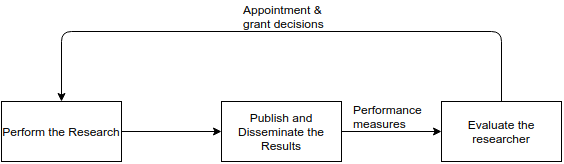
\includegraphics[width=12cm]{images/publication_process.drawio.png}
\caption{Publish for incentives (adapted from~\cite{BH2004})}
\label{fig:publish_incentives}
\end{figure}
% ==============================================================================

In this image we see that the researcher is evaluated and receives incentives 
(such as funds) based on performance measures. In their paper,  Bj\"ork and 
Hedlund mention that for public bodies that provide funds (which is an incentive 
for the researcher), the production and consumption of publications should be 
optimized.

Two main targets exists for the production part, (the scientific publication): 
journals (incollection) or 
conferences (inproceeding). While journal publications are the norm in many 
other disciplines, conference publications are common in Computer Science.

The next sections describe these processes from a Computer Science perspective. 
For other disciplines these processes may differ. For example, in CS 
conferences, rigorous peer-review is the norm, with acceptance rates of 20\% or 
less being common\footnote{Acceptance rates of security conferences: \url{http://jianying.space/conference-ranking.html}}; in other disciplines, such strict peer review for conferences is
less common.

% ==============================================================================
\section{Journal publication}

First we discuss the process for publishing in a journal. Although the 
exact process may differ across journals, there is a certain common process. We 
tend to describe this common process.

The process of publishing in a journal starts with the author who has a
manuscript he wants to publish. This can be based on a `call for papers', or on
own initiative. According to Cormode, the Editor-in-Chief receives the
manuscript and does a minor check if the paper is good enough for further
processing. If it is, the further process of handling the paper is assigned to
an associate editor 
who also performs some checks for quality (understandability, duplication of 
prior work, topic in scope). The checks from the editor-in-chief and associate 
editor can lead to a rejection of the manuscript. According to Cormode, the 
author is encouraged to suggest an associate editor at submitting~\cite{C2013}.
This helps the editor-in-chief to delegate the handling to a associate-editor 
with knowledge of the domain e.g..

The main responsibilities of the associate editor are 1) initial handling and 
selecting reviews for the papers and 2) obtaining a decision for a paper. 
Although selecting reviewers to review a manuscript is a responsibility of the 
associate editor, it is not uncommon for an author to suggest reviewers. 
Sometimes the author even needs to provide reviewers.

\begin{wrapfigure}{r}{0.27\textwidth}
    \centering
    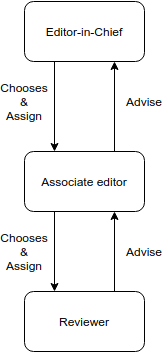
\includegraphics[width=0.27\textwidth]{images/c2013.drawio.png}
    \caption{Roles within the journal process (visual interpretation of description in~\cite{C2013})}
    \label{fig:c2013}
\end{wrapfigure}

After getting the results from the reviewers, the associate editor decides if 
the manuscript needs to be adjusted. Formally the reviewers give an advice, but 
it is up to the associate editor to do the final judgement. If adjustments are 
needed, the author adjusts his manuscript and this needs to be reviewed again. 
This can happen with other reviewers. An alternative path is that an author 
chooses to withdraw his paper.

Eventually, hopefully, if the paper is accepted by the associate editor, an 
advice will be given to the editor-in-chief. Formally the editor-in-chief 
decides if a paper is being published, but most of the time the advice of the 
associate editor is adopted. This chain of advice and assignment is shown in 
Figure~\ref{fig:c2013}. 

Interesting in this schematic overview is the absolute 
power of the Editor-in-Chief. The person in this role can make a judgement 
without the advice of the 
associate-editor (and reviewers). Also this role can influence the process by 
choosing a specific associate-editor. Under the Editor-in-Chief, we draw the 
Associate editor. This role has two ways to influence the process; by choosing 
the reviewers and by giving the advice to the editor-in-chief. The reviewers 
have less power; of course they can provide an advice, but in most of the cases 
there are multiple reviewers.

% ==============================================================================
To visualise the publication process for journals, we can use a model of 
Bj\"ork and Hedlund. They modelled the various processes involved in scientific
publishing to investigate the business impact of the shift towards internet
publishing models. This model is based on publication for journals. For our 
research, we took a diagram from their publication and took the activities 
usable for our research. Hereby neglecting the steps "Negotiate copyright" and 
"Copyedit Article". The result is shown in Figure~\ref{fig:bh2004_a22331}.

\begin{figure}[H]
\centering
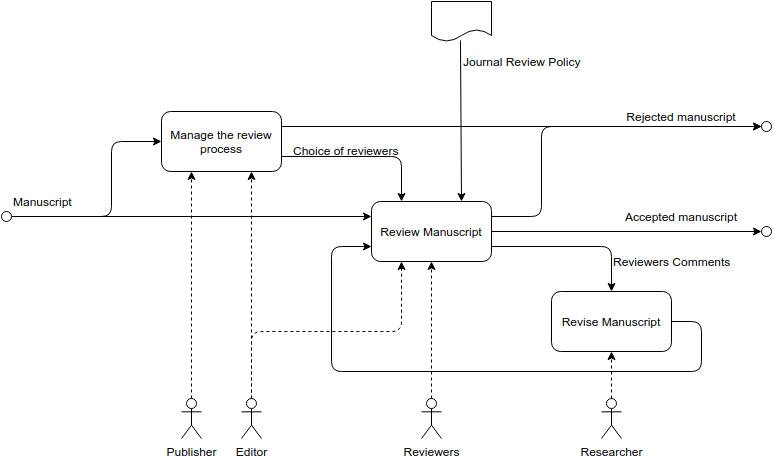
\includegraphics[width=\textwidth]{images/bh2004_dia_a22331_part.drawio.png}
\caption{Journal process flow between submission and decision (adapted
from~\cite[diagram A22331]{BH2004})}
\label{fig:bh2004_a22331}
\end{figure}
% ==============================================================================
The phase "Manage the review process" from Bj\"ork and Hedlund is described by 
Cormode from the perspective of the Editor-in-Chief and Associate editor (Bjork 
and Hedlund decided to use one role: editor). 

% ==============================================================================
\section{Conference publication}
The following is an informal description of the process for conference 
publication which can also be a workshop or symposium. Not all conferences 
follow this approach. Input for this description is provided by the supervisor
of this research project.

For established venues the steering committee decides to have a conference and 
choose a location. The main responsibility of the steering committee is to 
oversee the organisation of the conference and to choose the Program 
Committee (PC) chairs whose responsibility is to compose a program out of a 
subset of the received submissions. For new subjects, the trigger comes from one
or more academics who think a conference is needed for a certain subject and
try to form a Program Committee (PC). 

Possibly there are ``program tracks'' on specific subjects, with dedicated
chairs for each track.
% ============================================================================== 
The PC chairs invite people to become program 
committee members. A new trend is self-nomination; one can nominate himself for 
a position in the Program Committee. Another new trend is that authors of 
submitted papers are required to review.
Besides inviting members, the PC chairs ensure the website is up, promotion 
is in place and have submission/review server set up.

The PC chairs create and distribute a call-for-papers, which starts the 
\emph{submission phase}.
% ==============================================================================
Responding to the call-for-papers, scientists submit papers, and possibly 
marking conflict of interest. 
After a likely extension of the deadline, PC Chairs close submission and 
perform desk reject.
% ==============================================================================
After the submission phase closes the \emph{bidding phase} begins. During 
this bidding phase, PC members bid on which papers they would like to review.
In the \emph{review phase} the PC members read and score the papers. In this 
phase a paper can be early rejected with limited number of reviewers. Sometimes 
this phase contains a rebuttal phase; the reviews are sent to authors so the 
authors can reply on the given comments.

In the following \emph{discussion phase} the PC members unify their views about
the papers. After the discussion a decision should be made.
During the \emph{decision phase} the PC Chairs formalise a decision about a 
paper (formally; often they simply follow the consensus view). Possible 
decisions are accept, reject or conditionally accept (shepherding). In this 
case, the paper is interesting but not yet quite acceptable, salvageable. One 
reviewer is designated Shepherd and communicates with the authors on what 
changes are needed. Final acceptance hinges on the Shepherd officially 
approving the paper.

In the \emph{camera-ready phase} the authors make final changes, 
incorporating editorial changes, reviewer comments, etc., and submit the final 
version for publication.
In the \emph{publication phase} the PC chairs judge on the the camera-ready 
version, and papers is published online.
% ============================================================================== 


% ==============================================================================
\section{Fraud in the publication process}
\label{sec:domain_analysis:fraud}
% ==============================================================================
In the introduction we already referred to the aphorism known as Goodhart’s Law 
: ``When a measure becomes a 
target, it ceases to be a good measure''~\cite{strathern_1997}. Known metrics 
such as the H-Index (a performance metric for researchers) not only incentivise 
scientific excellence; they also invite other ways to achieve high rankings 
(e.g. plagiarism, manipulation of images, manipulation of research data, 
fabrication of research data). 
% ==============================================================================

This section provides short description of some interesting cases that may 
occur in the above described processes.
It is certainly not the case that all situations do actually imply fraud, but 
these are cases that are a candidate for further manual investigation.
Here we do not mention content-based fraud like plagiarism, we focus on fraud
during the publication process. As Mario Biagioli calls them `post-production 
misconduct', which is probably a nicer term~\cite{biagioli2020gaming}.

\paragraph{Publications cites publications in the same venue} It is remarkable
if a venue cites only work from itself. The benefit for this venue is that it
increases the impact score of the venue. This case is described as an example in
Section~\ref{interesting_case:publications_cites_publications_in_same_venue}.
% ==============================================================================
\paragraph{Work member of editorial board is being cited} Member of the
editorial board that is excessively often being cited in his own venue, can be
an indicator for fraudulent behaviour. This case serves as input for case 
study~1 (Chapter~\ref{chp:case1}) and is described further in 
Section~\ref{interesting_case:work_member_editorial_board_cited}.
% ==============================================================================
\paragraph{Member of the editorial board is (co-)author} 
A questionable situation occurs if a member of the editorial board becomes 
co-author of \textit{relatively} a lot of publications. This may indicate that 
authors are being forced to add the member to the author list. The benefit for
the member is an increased publication count and, if the article gets cited, 
citation count (which has impact on the H-Index and therefore impacts his 
career). This situation is described in case study 2
(Section~\ref{interesting_case:member_editorial_board_is_coauthor}).

% ==============================================================================
\paragraph{Author reviews his own work}
This kind of fraud is known because of Moon. Moon gave an e-mail address of 
himself (alias) as reviewer for his own work. This case was detected because of
the short time between submission and accordance. Moon was detected, but are 
other authors that show this fraudulent behaviour also detectable?
Case study 3 (Chapter~\ref{chp:case3} is based on this publication-lag (time 
between submission and publication of an article).

\ \\
Of course possible fraudulent behaviour is not limited to these cases. Other 
cases are described on the website of COPE (Committee on Publication
Ethics)\footnote{\url{https://publicationethics.org/guidance/Case}}.

\section{Conclusion}
In this chapter we described the processes to publish articles for journals and
conferences. In these processes fraud can be conducted, which we have shown with
a few cases. The information in this chapter is domain knowledge which is needed
to conduct this research.

% ==============================================================================
\chapter{Related work}
\label{chp:related_work}
% ==============================================================================

As stated in the introduction a more generic approach for fraud detection is 
needed. This research is a continuation of the research of Tielenburg, which
tried to apply this generic approach~\cite{TEJ2017}.

\begin{wrapfigure}{r}{0.25\textwidth}
    \centering
    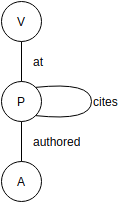
\includegraphics[width=0.25\textwidth]{images/jm2017_undiced_pub_view.drawio.png}
    \caption{Set-theoretic publication model adapted from~\cite{JM2017} used 
by~\cite{TEJ2017}}
    \label{fig:rw_jm2017}
\end{wrapfigure}

Tielenburg investigated automated detection of fraud-like behaviour based on
publicly available data ga\-thered from DBLP and Google Scholar. He determined 
fraud indicators based on a data model of the publication process proposed by 
Jonker and Mauw~\cite{JM2017} shown in Figure~\ref{fig:rw_jm2017}. In this 
model \textit{V}, \textit{P} and \textit{A} stand for Venue, Paper and Author.

Tielenburg proposed three heuristics calculated about the authors to identity 
outliers: 
\textit{maxdiffpubcount} (maximum over the difference in the number of 
publications between two consecutive years), \textit{maxdiffcitecount} (maximum 
over the difference in the number of citations between two consecutive years) 
and \textit{maxratiocitsvspubs} (maximum of the ratio between citations and 
publications). The latter is a derived value based on publication 
and citation counts per year.

Tielenburg's implementation based on the data modelled by Jonker and Mauw was 
not successful; entities (e.g. the reviewer) are missing in this model. 
Therefore, this model needs to be extended.

\paragraph{Extending the model}
Haug raised attention to fraud in the peer-review process and the important role
(guest-)editors have in relation to the peer review process~\cite{Haug2015}. The 
attacks she presents are self reviewing like Moon and Chen and fake reviewers.
Another attack she mentions is the attack on the systems supporting the peer-review
process.

Bishop\footnote{\url{http://deevybee.blogspot.com/2020/07/percent-by-most-prolific-author-score.html}}
additionally considers the impact of the role of the editor.
In her blogpost she raises attention to members of the editorial board which are
also co-authoring articles. However, this is mainly focuses on one editor.

Scanff et al.~\cite{SNCMBL2021} focused on the publication process of prolific
authors, who might be part of the editorial board. They measured the
publication time (time between submission and acceptance) of these prolific
authors and noticed how this period is less for papers written with prolific
author compared to papers written without prolific authors. 


\paragraph{Available datasets}

\emph{\dblp{}} is a publicly available dataset focused on publications in the
Computer Science Domain. The dataset contains publications, authors and venues.
Ley describes the choices made by \dblp{} composing the
dataset~\cite{DBLP:journals/pvldb/Ley09}. The person entity is described in 
detail included the procedure DBLP takes to identify unique people with the same
name or an author with multiple names.
The data \dblp{} uses to create this dataset is being pushed from publishers or 
scraped from the web using web crawlers. \dblp{} covers the datamodel of Jonker
and Mauw without the citations.

Heibi et al. introduced the \emph{OpenCitations} COCI (Crossref OpenCitation 
Index) dataset. This dataset contains citations on DOI-to-DOI
based~\cite{DBLP:journals/scientometrics/HeibiPS19}.
OpenCitations acquired their data from undisclosed datasources.

Aminer is a service that provides datasets for analysis of the publication
process.
Tang et al. descibed how \emph{Aminer} loads the source data from sources and 
uses probablistic models to deal with name disambiguity~\cite{Tang:08KDD}. As 
with DBLP, Aminer also elaborates on how they tackle the author-naming problem.
The citation dataset, which contains authors, publications and citations, uses
data from DBLP, ACM and `other sources'. 
Aminer covers the model from Jonker and Mauw, focused on citations. For the 
entities involved, a lot of attributes are not available.

These datasets are not complete. Chakraborty et al.~\cite{CPN2021} found 
data on the various
roles in the publication process lacking to such an extent, they could not complete
their originally envisioned research. Thus, while specific roles may significantly
impact the publication process, data regarding these roles is not readily available.
Data acquisition is thus a key component of any study into the correlation between
specific roles and impact.
Therefore, acquisition of additional data is needed.

\paragraph{Data acquisition and parsing}
As described in previous paragraph, the actual source data used to create public
datasets is not transparent. However, generally we notice that the most
`original' data (not acquired from other public datasources) is acquired from
websites of publishers (e.g. using the webcrawlers in case of \dblp{}). 
Besides websites, publications and editorials are most of the time available in
PDF format. Therefore we focus in this paragraph on acquisition which contains
`downloading' the content (which may be HTML of PDF) and parsing, transforming
the acquired data in information.

For downloading content from the web (e.g. HTML or PDF documents) standard
tooling exists (e.g. cURL\footnote{\url{https://curl.se/}},
wget\footnote{\url{https://www.gnu.org/software/wget/}}). For incorporating this
downloading in software, multiple libraries exist.
In case of HTML two types of methods for acquiring content exist: web browser
wrappers (e.g. Selenium) and HTTP libraries (e.g. Urllib2)~\cite{zhao2017}. The
first simulates a browser. The advantage is that dynamic content can also be
acquired. The second is a single GET request (which is equivalent to tooling
described before).
The content acquired differ from site to site. Therefore, this content needs to
be interpreted to turn this acquired data into information.

\ \\
Parsing is extracting information from the acquired (raw) data. The parsing 
mechanism depends on the type of data.  Examples are HTML (web pages), datafeeds
in XML and JSON or multimedia types. Considering the type of data his research 
is conducted on, we focus on HTML and PDF files.
Zhoa~\cite{zhao2017} mentioned BeautifulSoup for interpreting HTML and Pyquery
for XML. Uzun et el.~\cite{uzun2018comparison} comparised regex and DOM-based 
libraries (Lxml and BeautifulSoup) for data parsing. DOM-based libraries were 
better for parsing than using regex.
Lo et al. interpreted PDF's from multiple papers \cite{lo-etal-2020-s2orc} to 
extract bibliographic information. They also tried to parse Latex documents, but
surprisingly, the results were worse with Latex then with PDF. For extracting 
information from PDF's, they relied on a project called
ScienceParse~\footnote{\url{https://github.com/allenai/science-parse}}. This is 
framework that interprets Scientific Papers. The main component used to read the
PDF documents, is PDFBox.
This parsing of PDF's is similar to \cite{niu2014realization} and \cite{BK2017}.
Bast and Korzen performed a benchmark of tools for extracting text from PDF 
documents. Considering the error-rate of various tooling, pdftotext, pdftohtml, 
pdftoxml, pdfbox and parscit are considered the top 5 tools~\cite{BK2017}


% Niu et al. also extracted information from papers \cite{niu2014realization}.
% For extracting text from PDF's multiple studies are conducted for interpreting 
% scientific papers \cite{niu2014realization}, \cite{BK2017}.
% Bast and Korzen performed a benchmark of tools for extracting text from PDF 
% documents. Considering the error-rate of various tooling, pdftotext, pdftohtml, 
% pdftoxml, pdfbox and parscit are considered the top 5 tools~\cite{BK2017}.

% Hashmi et al. provided an overview with possible methods to extract 
% information from the text. They describe the Machine Learning, Rule-based and 
% hybrid approaches \cite{hashmi2020insights}.



% ------------------------------------------------------------------------------
\paragraph{Modelling the publication process} \label{rw_publication_process}
% ------------------------------------------------------------------------------
For integration of multiple datasources, we need a model of the publication 
process.
We already mentioned the set-theoretic publication model presented by 
Jonker and Mauw~\cite{JM2017}, shown in Figure~\ref{fig:rw_jm2017}. This model
is used to formulate an attack surface on the publication process. However, 
based on work from Tielenburg, Haug, Scanff et. al. and Chakraborty et al. we 
can conclude that this model does not represent the necessary information.

% ==============================================================================
Björk and Hedlund~\cite{BH2004} describe a  model of the publication process
for measuring costs. Their model includes a large set of involved entities
and roles. While this model provides a solid foundation for understanding the
publication process, the model is a process model and does not facilitate
deriving publication metrics. As such, it is unsuited for determining
the value of quantified fraud indicators.

% ==============================================================================
From the view of the associate-editor, Cormode describes in detail how his work
looks like~\cite{C2013}. It provides a good insight of the work of an associate 
editor, which can also be read from an 'attacker-mindset' (where are the 
vulnerabilities), but unsuited for fraud detection.


\paragraph{Data integration}
After acquisition and parsing, the data needs to be integrated. This integration
is a common step in ETL (Extract Transform Load). ETL is known as a process
used in data warehousing (component to serve historical data formatted
for reporting and analytics). Therefore, most integration techniques come from
this area of expertise. Physical datamodelling techniques are Data
Vault~\cite{linstedt2015building} and Anchor
modelling~\cite{ronnback2010anchor}. Both are ensemble modelling techniques;
this means focusing on a business level (business entity based) and an agile
approach (the model can be changed and grow incrementally). An important aspect
of these techniques is the availability of a cross-source key (business key) to
match the same objects from different sources. These physical datamodelling
techniques can be used in the implementation phase of our study, if such
cross-source keys can be identified and the quality is acceptable.
For example, in the domain of scientific publication, this role could be filled
by \doi{}\footnote{Digital Object Identifier, an identifier intended to uniquely
identify a scientific publication.} or \orcid{}\footnote{Open Researcher and Contributor
Identifier, an identifier intended to uniquely identify people involved in scientific
publications.}, if used in all sources. 

% ==============================================================================
\chapter{Methodology}
\label{chp:methodology}
% ==============================================================================
In Chapter~\ref{chp:domainanalysis} we described the processes to publish 
articles for journals and conferences. In these processes fraud can be conducted.
%
To improve detection of this fraud, data about these processes is necessary.
Previous approach (\cite{TEJ2017}) to discover fraudulent behaviour was based 
on public datasets, but misses important entities. 
%
Considering the cases described in Section~\ref{sec:domain_analysis:fraud} and 
public datasets that are generally represented by Jonker and Mauw~\cite{JM2017},
missing entities can be pointed out.
In Figure~\ref{fig:jm2017_missing_ent} the generic data model for public 
sources is on the right side; V for venue, P for paper and A for author. Left of
this model some missing entities are added.


\begin{figure}[H]
\centering
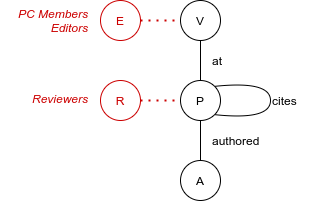
\includegraphics[width=7cm]{images/jm2017_miss_ent.png}
\caption{Right: Set-theoretic publication model adapted from~\cite{JM2017} Left: Missing entities considering example attacks.}
\label{fig:jm2017_missing_ent}
\end{figure}

% ============================================================================
However, these missing entities are available, but not in a structured format 
and integrated in existing datasets. Our assumption is that integrating 
additional data will improve directing manual effort in detecting fraudulent
behaviour. This brings us to the main question of this research:

\ \\
\begin{center}
\textbf{To what extend can integration of publicly available data sources 
contribute \newline to directing manual investigation of scientific fraud?} \\
\end{center}

\newpage
\section{Method}
On a high level, this is a two step process:
\begin{enumerate}
    \item Define the datamodel for the publication process;
    \item Acquire and integrate data to fill this datamodel.
\end{enumerate}

% ============================================================================
\paragraph{Define datamodel}
Missing entities are mentioned in the problem described in the lead of this 
chapter. The resulting figure (Figure~\ref{fig:jm2017_missing_ent}) is not 
sufficient to build a dataset for fraud detection. Therefore, as first step a 
more concise datamodel is needed to enable detection of interesting cases. 
With this step we identify entities and their relations. Possible approaches 
to define a datamodel are:
\begin{itemize}
    \item \emph{Use an existing datamodel}: Datamodels about the publication 
    process do exist. An initial analysis made clear that existing models are
    somehow limited to the author, venue and publication. Attacks as described
    in Section~\ref{sec:domain_analysis:fraud} are not possible to detect using 
    these models. As an example: the Microsoft Acadamic Graph 
    model\footnote{\url{https://docs.microsoft.com/en-us/academic-services/graph/reference-data-schema}} 
    (which is the most detailed we came across) does not contain any other role 
    than author.
    \item \emph{Create a model}:  The domain analysis can be used as input to create
    a datamodel.
\end{itemize}

A combination of these approaches will add the most value for this study. The 
reason is that existing models are a good starting point. However, some 
extensions are needed for our study. We scope this step by modelling a logical 
model. There are two reasons for this:
\begin{enumerate}
    \item A physical model containing all possible attributes is too 
        detailed. Taking this approach will take too much time while the added
        value is not worth the effort.
    \item By using a logical model, the focus is on the entities and their
        relations. These are the most important components for a group based
        detection.
\end{enumerate}
% ============================================================================
This does not neglect the need for a physical model for implementation. 
Multiple physical modelling techniques exist which can be used for 
implementation.
% By using a more high-level logical model approach, we can define a model 
% focused on the entities and relations involved, which can be implemented 
% using multiple physical modelling techniques. 


\paragraph{Acquiring and integrate data}
The second step is to determine which publicly available dataset can (partially)
fulfill some parts of the model defined in the previous step. Our approach is
here to discuss the available datasets and how these cover the model.
Based on the research preparation, we know \dblp{} and Aminer are two sources
that we probably can use. In this step a more extensive investigation is 
needed focused on integration and covering entities and relations from the 
resulting model from the first step.
Sources for required entities not covered by public datasets should be found. 
For every source we should investigate the following points:

\begin{itemize}
    \item How the acquisition will take place. This depends on the source.
    \item How integration of this newly acquired data should take place. This 
        depends on available attributes.
\end{itemize}

An approach for these added sources can not be decided up front.

% ============================================================================

\section{Validation}
As we know from our research proposal, publicly available datasets do not 
contain necessary information to identity groups. Therefore, data to apply 
group identification needs to be acquired from additional sources and 
integrated with other existing datasets. Detect outliers within such groups
which can be used to direct manual investigation, proves the added value of 
integrated data.

\paragraph{Apply group based outlier detection}
In this step we define groups and apply a group based detection on the dataset
composited from the previous step.
In the domain analysis of the 
publication process interesting situations are 
described with the groups having the power to abuse that particular situation
(Section~\ref{sec:domain_analysis:fraud}). In Figure~\ref{fig:research_method} this
is these are represented with the arrows from the publication process to the roles.

\begin{figure}[H]
\centering
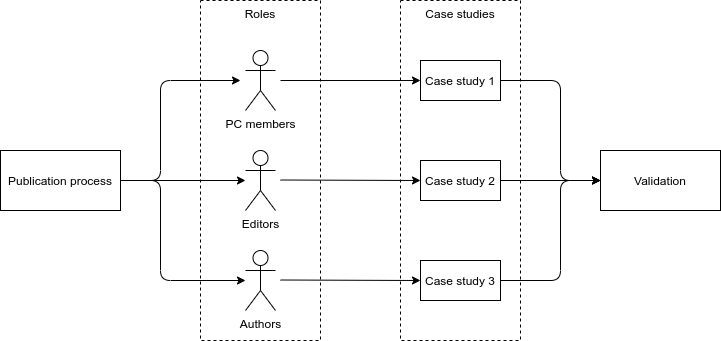
\includegraphics[width=13cm]{images/research_method/research_method.png}
\caption{Relation publication process, roles and case studies}
\label{fig:research_method}
\end{figure}
Based on these situations three cases studies (identifiable groups) are formulated:
\begin{itemize}
    \item Program Committee Members
    \item Editors of a journal
    \item Authors based on publication lag
\end{itemize}

For every use case we do the following:
\begin{itemize}
    \item Create an analysis dataset from the previous step focussed on this
    group and its metrics;
    \item Validate possible interesting cases.
\end{itemize}

\paragraph{Formalising the conclusion}
The combinations of validations from the case studies will result in the
answer on the question to what extend the integration of publicly available data 
sources contributes in directing manual investigation of scientific fraud.

% ==============================================================================
\chapter{Data model and standard data sets}
\label{chp:data}
% ==============================================================================
In this chapter we describe the underlying data model to perform group based 
outlier detection. This chapter addresses three points:
\begin{itemize}
    \item The ideal data model for the publication process;
    \item Known data sources to fill this data model;
    \item Completeness of these known sources to fill the data model.
\end{itemize}


\section{Ideal data model}
By formalising the ideal data model, we can answer which entities and which 
roles are involved and their relationships.
The ideal situation is one dataset which contains all entities and relations 
and can serve as base to easily create the necessary datasets upon to perform 
group based data analysis. As 
input to reason about this dataset we use the domain analysis from 
Chapter~\ref{chp:domainanalysis}.
As starting point: Jonker and Mauw formalised the publication
model~\cite{JM2017} 
and created an entity based view of the publication process. 
Figure~\ref{fig:jm2017_induced_pub_model} depicts their final model.

\begin{wrapfigure}{r}{0.25\textwidth}
    \centering
    \vspace{-15pt}
    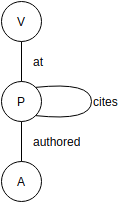
\includegraphics[width=0.25\textwidth]{images/jm2017_undiced_pub_view.drawio.png}
    \vspace{-13pt}
    \caption{Set-theoretic publication model of papers (P), venues (V), and 
authors (A) (adapted from~\cite{JM2017})}
    \label{fig:jm2017_induced_pub_model}
    \vspace{-16pt}
\end{wrapfigure}



% ==============================================================================

Whereas the Jonker and Mauw only modelled the author as a role in the process, 
Bj\"ork and Hedlund mention the publisher, editor and reviewer as well. 
We consider the author from Jonker and Mauw the same as the researcher from 
Bj\"ork and Hedlund. In this research, we ignore the publisher. Although the 
publisher is responsible in the end and sets the regulations and constraints for
editors to work within, the actual work is delegated to editors.

Extending the model of Jonker and Mauw with the description of Cormode
\cite{C2013} results
in a model that incorporates the most important roles with influence on the 
judgement of the work of an author. We 
ignore roles like the editorial assistance and subeditor, because these roles do
not seem to have influence on the judgement of a manuscript. 

In Figure~\ref{fig:structure_journal} we provide an overview of the entities and
roles from Jonker and Mauw combined with the information from Cormode which 
answers the roles involved and their dependencies.
The red rectangles are objects and the green circles are roles.
As objects we have a venue which contains papers. Multiple roles are related to
these objects.

\begin{figure}[t]
\centering
\includegraphics[width=11cm]{images/chp_5/set_theoretic_model_of_pub_process_collections.png}
\caption{Set-theoretic model of the publication process for collections.}
\label{fig:structure_journal}
\end{figure}

It is important to notice that the green circles are roles, not entities. These 
roles are fulfilled by people. This results in one more entity (person) with 
relation to other entities. These relationships can be expressed as the roles 
(e.g. a person is a reviewer for a publication).

% ==============================================================================
\subsection{Conferences}
So far we only focused on the process of journals. But, as mentioned before, 
publishing for a conference is important in the Computer Science domain.
In case of conference publications, the author, publication and its relation to 
the venue stay the same. It is possible that this venue becomes more extensive 
because of tracks, but it stays a venue.
An important person for conferences is the Program Committee Member. Eventually
this is again a role of a person related to the venue.

% ==============================================================================
\subsection{Resulting model}
\label{sec:resulting_model}
In the resulting model we choose to abstract the roles away and use one entity 
called person where we define the roles to certain entities in the relationship.
This makes the model far more easy to reason about when a person has multiple 
roles.

The model in Figure~\ref{fig:resulting_model} is a logical model. A physical
model can be designed based on this logical model using design
strategies like Ensemble Modelling (e.g. Data Vault~\cite{linstedt2015building}
or Anchor modelling~\cite{ronnback2010anchor}). Which
modeling principle is being applied is not important. What is important, is that
the physical model address requirements like time-awareness and tracking changes
of entities to create a physical model. E.g. a person is not 'always' 
editor of a venue, this role starts and stops at a certain moment in time.
\begin{figure}[t]
\centering
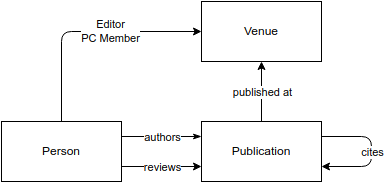
\includegraphics[width=9cm]{images/set_model.png}
\caption{Set model which covers necessary entities and relationships}
\label{fig:resulting_model}
\end{figure}

% ------------------------------------------------------------------------------
\subsection{Example: Publications cites publications in same venue}
\label{interesting_case:publications_cites_publications_in_same_venue}
In this part we will go through a situation to describe the process of analysing
a situation which can be an attack on the publication process and plot this on the
resulting datamodel from the previous section. The chance this 
particular situation occurs is not very high. The reason is that there is a good
enough safety net to catch this situations provided by Thomson Reuters\footnote{\url{https://clarivate.com/webofsciencegroup/solutions/journal-citation-reports}}, 
institute that 
calculates the Journal Impact Score. Besides, in our research we are looking for
interesting people. Because this description method of an interesting case is
used later in this thesis, description of the steps taken are added. 

\textit{First we describe the situation and provide a model of instances that 
are involved. This can be a person in a certain role, venues, publication etc}.

Having publications citing publications from a certain venue, increases the 
journal impact factor.
Figure~\ref{fig:cpsv} is a model of this situation; a venue (v1) that
contains a publication (p1) which has a citation (c1) to a publication (p2) in
the same venue. As an example to clarify the notation, p1 and p2 are both 
different instances of a publication; we will use this notation when we describe 
other cases as well.

\begin{figure}[ht]
\centering
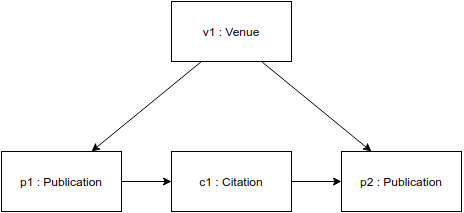
\includegraphics[width=9cm]{images/cited_publications_same_journal.drawio.png}
\caption{Instance model of citation of publication in the same venue}
\label{fig:cpsv}
\end{figure}

% ------------------------------------------------------------------------------
\paragraph{Attack}
\textit{We describe when (this is not always the case, see 'Benign 
alternatives') and how this situation is an attack.} 

It is not unusual that publications in a journal cite publications from the same
venue. However, as with most attacks, when this occurs much more compared with
other venues and the 'inner venue'-citation rate is significant higher, it
becomes interesting. This may indicate that this is a conscious action to
increase the Journal Impact Score, and this can be considered an attack.

\paragraph{Model impact}
\textit{In this part we describe how this situation impacts the publication 
model. What does in- or decrease and how does this impacts the 'score' 
of the attacker.}
The impact on the publication model is that the number of citations to 
publications in the same venue raises. Therefore, the impact score of a journal
raises. 

\paragraph{Benign alternatives}
\textit{In this part we describe how this situation can occur, while not being
an attack.} 

If a certain venue is that specialised in a certain topic, the 
situation where a publications cites other publications in that venue can occur.


% ==============================================================================
\section{Publicly available datasets}
\label{sec:data_public_datasets}
In this section we will explore some publicly available datasets with the focus 
on Computer Science which can be used to fill the model from
Section~\ref{sec:resulting_model}. Because of the necessary ability to integrate
datasets, we will judge these sets on integrability and completeness.
As a guideline, we will use Figure~\ref{fig:dataflow_jm2017_a}. Our main target
is to create a publication view based on the data sources which are represented
in the figure as `raw data'.
\begin{figure}[H]
    \centering
    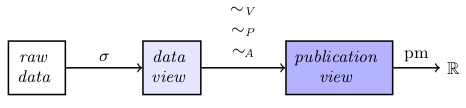
\includegraphics[width=10cm]{images/data_to_publication_metrics_jm2017.png}
    \caption{Data flow (\cite{JM2017})}
    \label{fig:dataflow_jm2017_a}
\end{figure}

The sigma-sign represents the filter on the set. For now, this filter sets the 
focus on the Computer Science area. Later on, this filter can be more 
strict, depending on the case study.
The tilde-sign is to combine multiple representations of the same object from 
sources to one object (e.g. a paper available in two different datasets is 
represented by one paper in the publication view).
Futhermore, the pm is a `publication metric'-function resulting in metrics 
(e.g. number of citations).

A known datasource for Computer Science in DBLP. We can use this dataset as base.
For other research areas, other datasources should be taken (e.g. for 
biomedical research, one can use PubMed).

% \begin{itemize}
%     \item Publicly available sources are limited in available data. Most datasets provides information on who wrote what and sometimes which article refers what. This provides a good insight and based on these datasets a lot of research is already conducted.
%     \item However, we think these datasets miss actors on the publication process that are in a position with enough power to influence the publication process.
%     \item Data about these people involved in the publication process are not structured available to use in analysis. The information is provided in front matters and masthead documents. Because of the nature of these documents, mostly PDF's, we consider this as unstructured data.
%     \item We are somehow surprised of the lack of structured data availability about these people, because of their power and influence.
%     \item Our focus in this chapter is to incorporate this less structured available data into publicly available data about the publication process to get a dataset which provides a more complete view of the publication process.
%     \item Our research focus on information technology so our start point to gather these people is to use the most prominent conferences and journals. As source for this data we use the core ranking.
% \end{itemize}

% \outline{
% \begin{itemize}
%     \item Model wat in dblp, aminer en in HJ staat
%     \item Model publicatieprocess
%     \item Sluit niet aan
%     \item meer rollen -> niet in publieke datasets
%     \item Most public available datasources for the publicationprocess contain information about the author and what the author publishes. Sometimes (but not all, or incomplete) these datasets also contain references.
%     \item The model of these datasets are visualized by the publication process of Jonker and Mauw.
%     \item Examples of these datasets are DBLP and Aminer.
% \end{itemize}
% }


% ==============================================================================
\subsection{DBLP}
\label{sec:data:dblp}
DBLP is a dataset with bibliographic information in the computer science 
discipline which can be downloaded in XML format. In 
Figure~\ref{fig:set_model_dblp} we show which elements of the set are 
covered by DBLP.

\begin{figure}[H]
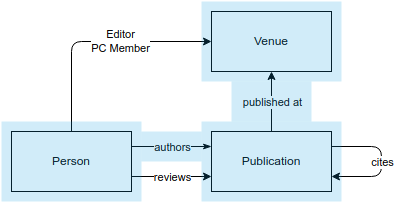
\includegraphics[width=9cm]{images/set_model_dblp.png}
\centering
\caption{Set model DBLP}
\label{fig:set_model_dblp}
\end{figure}

% \outline{
% \begin{itemize}
%     \item Structure of delivery
%     \item Processing
%     \begin{itemize}
%         \item convert XML to relational tables
%         \item Every bibliographic type in separate table
%         \item Assign unique id
%         \item Make separate table for elements with id of bibliographic record
%         \item Attributes of elements are columns in table
%         \item Add metadata to all data entries
%     \end{itemize}
%     \item Result
%     \begin{itemize}
%         \item 35 tables
%         \item overzicht van tabellen en relaties
%     \end{itemize}
% \end{itemize}    
% }

Unfortunately DBLP misses some important information to be complete; the dataset
does not contain references, editors, PC members and reviewers. For 
references, other sources can be addressed: Aminer, OpenCitations or Google 
Scholar.

% ==============================================================================
\subsection{Aminer}
Aminer positions itself as an AI for academic publications~\cite{Tang:08KDD}. 
One dataset they provide is the 
'Citation Network Dataset'. This dataset combines data mainly from DBLP, ACM (a 
publisher) and MAG (Microsoft Academic Graph). Because it uses DBLP as a 
source, it is interesting to 
investigate if we can use this for filling the gap of the citations shown in 
Figure~\ref{fig:set_model_dblp}.
In Figure~\ref{fig:set_model_aminer} we presented which entities and roles
from our ideal data model this dataset contains. Although this set contains data
from these entities, the attributes are limited; the main purpose of this set is
citations.
\begin{figure}[H]
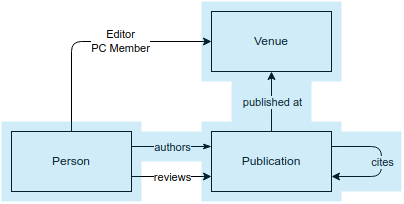
\includegraphics[width=9cm]{images/set_model_aminer.png}
\centering
\caption{Set model Aminer}
\label{fig:set_model_aminer}
\end{figure}


\subsection{OpenCitation} 
OpenCitation is a \doi{} based reference dataset. This means, the cited and citing 
articles are referred to by a \doi{}. 
The dataset from opencitation can be downloaded, or questioned by an \api{} request. 

From the publication entity it only contains the \doi{}.


\subsection{Google Scholar}
\label{subsec:google_scholar}
Google Scholar also contains the references from and to articles. This data is 
only available online. Some software packages exists that support scraping this
information. However, experiments from the research preparation phase concluded
that this was not a feasible solution because of the amount of captcha's when
trying to scrape the site. The acquisition of this data is not practical.

\subsection{Conclusion data availability}
\label{subsec:ConclusionsDataAvailablity}
Referring to the ideal model as given in Figure~\ref{fig:resulting_model}, we 
can make a few statements:
\begin{itemize}
    \item The availability of data about publications, venues and authors is 
    good; almost all public sources contains some information about these 
    entities. 
    \item References are available in two publicly available sources (we ignore 
    Google Scholar for given reasons in Subsection~\ref{subsec:google_scholar}).
    \item Other roles than `author' are not available in public datasets.
\end{itemize}

In the next section we will investigate how these sources can be integrated.

% \section{Deviation publication model and available data}
% As visualised in Figure~\ref{fig:set_model_dblp} and Figure~\ref{fig:set_model_aminer}, both datasets miss some crucial roles.
% Both sources miss the reviewer, editor and PC Member. These roles are crucial in the publication process and are a must-haves in our group-based outlier detection.

% This raises the question where we are able to get this data. Luckily, there are is some data about these roles publicly available, but this is not straight forward. We will come back to this point when we describe the case studies.

% ==============================================================================
\section{Integrability}
\label{sec:data_integrability}
People, articles and venues can be acquired from multiple source. To be able to 
work with these entities, we need to integrate these sources in one model. To 
make this possible, we need to uniquely identify the entities.
In the ideal situation entities have an unique identifier which is 
independent of the source. However, in practice it is a bit more complex than 
that.

% ==============================================================================
\subsection{Articles}
The unique key which is used to identity an article is the Digital Object 
Identifier. This field is available in DBLP, Aminer and OpenCitations. Also, the
\doi{} should be unique across all articles. 
Theoretically, combining the sets using the DOI should be possible without much
effort.
However, an analysis of the DBLP data set leaves us with a few DOI's which refer
to multiple articles. The number of articles this occurs, is very low
(approximately 20 articles; a manual override is a possibility). Also, DBLP 
has a lot of documents where the DOI is unknown; so data completeness 
is an issue here. 

\subsubsection{DOI Availability}
\label{subsec:data_doi_availability}
\emph{DBLP} contains additional information about an entry in an ee tag. These contain 
links to doi.org, wikidata, etc. Sometimes an article has multiple doi.org links; 
this seems mostly the case with the publisher ACM. Although the links are 
different, they redirect to the same page at ACM.
For articles the following count of DOI's is available.
\begin{center}
    \begin{tabular}{ rr }
        \toprule
        \# of DOI & \# of articles \\
        \midrule
        0 & 1,051,229 \\
        1 & 4,626,193 \\
        2 & 22,396 \\
        $\geq$ 3 & 1,202 \\
        \bottomrule
    \end{tabular}
\end{center}

Concluding; most articles do have a \doi{}; approximately 78\% has one or multiple 
\doi{}'s.

% ==============================================================================
\emph{Aminer} provides one \doi{} field for an article. Also not all DOI's are
available. For the 4894081 articles in Aminer, 3920939 has a \doi{}
(approximally 80\%). However, the \doi{}'s provided in the dataset are not
unique: 3316 DOI's are used to identify multiple articles. A quick investigation
taught us that Aminer 
sometimes uses a \doi{} to refer to a journal instead of an article. Another 
finding with a quick analysis in the case of \doi{}'s, is that multiple articles
are represented multiple times in the dataset; the article dataset is not 
unique. This raises some doubt about the quality of the dataset of Aminer.

\subsubsection{Alternative key}
Because the \doi{} is not a useful key across all sources to integrate data 
because of availability and uniqueness, alternative fields that make a good 
candidate to serve as key are looked into. 
A combination of title, authors, year and journal makes a good candidate.
% ==============================================================================

The title and how sources save this title may differ. 
Sometimes the sources uses other characters. For example, \dblp{} uses an HTML
tags to specify characters in the title, e.g. see 
Listing~\ref{lst:DblpTitle}. This in combination 
with specific symbols (e.g. Greek delta-sign) which are expressed differently 
depending on the source, makes joining sets on titles with these signs
cumbersome.

\lstset{language=XML}
\begin{lstlisting}[caption={Example title in \dblp{}},label={lst:DblpTitle}]
<title>Graphs of Bounded Treewidth can be Canonized in AC<sup>1</sup>.</title>
\end{lstlisting}

These problems can be overcome by applying some clean rules before the join. 
Considering a solution for the title exists, still a join on other attributes
needs to be done; the title itself is not unique.
Which raises a next integration problem: people.

% ==============================================================================
\subsection{People}
\label{sec:integrability_people}
In the publication domain an identifier for a person exists, this is called
the Open Researcher and Contributor ID (\orcid{}). This field is (partially) 
available in \dblp{}, but not in Aminer.
Alternative approach to uniquely identify authors is the name. However, this has
multiple issues:
\begin{itemize}
    \item \emph{Format}: A name can be written in multiple formats. E.g. a person is 
    named Alfred Jodocus Kwak; this can be written as `Alfred Kwak', 
    `Alfred J. Kwak', `A. J. Kwak', `A. Kwak' and of course the full name. 
    With names that contain accents on letter, the possibilities increases.
    Also, in some countries it is used to put the family name first.
    \item \emph{Multiple people with same name}: The name does not make an author 
    unique. The same name refers to other authors. 
    \item \emph{Other names for the same person}: E.g. when Robert is also called Bob.
\end{itemize}

Both \dblp{} and Aminer acknowledge this problem. In case of multiple 
people with the same name, DBLP addresses this problem by suffixing the
name with a four digit code\footnote{\url{https://dblp.org/faq/1474704.html}}.
\dblp{} is making progress here, but this is not entirely done yet. 
The format issue and alias issue is covered by \dblp{} by creating a master 
record for the author, see Listing~\ref{lst:DblpAuthorMasterRecord} as an 
example.
Aminer uses an approach which takes the coauthors in to account. It creates
a network of co-authors for a certain author and then calculates a 
probability that this is the same author.

However, an exploratory analysis of the \dblp{} data makes clear this is not 
flawless; cases exist where the same master record authors one 
article multiple times. After a small investigation it seems that a father 
and son both authored this article (Robert and Bob, same lastname so \dblp{} 
'chooses' to treat these names as the same person).
% ==========================================================================
\lstset{language=XML}
\begin{lstlisting}[
caption={Example master record(\url{https://dblp.org/faq/1474690.html})},
label={lst:DblpAuthorMasterRecord}
][h]
<www key="homepages/r/CJvanRijsbergen">
<author>C. J. van Rijsbergen</author>
<author>Cornelis Joost van Rijsbergen</author>
<author>Keith van Rijsbergen</author>
<title>Home Page</title>
<url>http://www.dcs.gla.ac.uk/~keith/</url>
</www>
\end{lstlisting}

But hypothetically, even if \dblp{} manage to unique identity authors, 
the match to authors in other datasources is not possible, if these sources 
do not adhere the same method.

% \subsection{Article integration}
% Not only do we need to match the articles of DBLP and Springer LNCS, we also 
% need to incorporate Aminer. Aminer is an enrichment of DBLP in that it adds
% citations. Although DBLP is working to incorporate citations in their dataset,
% this is still work in progress and Aminer has already a lot of that data.

% \begin{figure}[H]
%     \centering
%     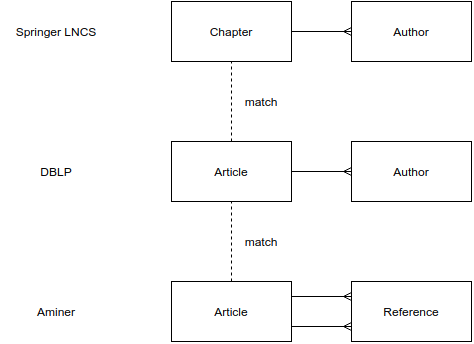
\includegraphics[width=10cm]{images/linking_article_dblp_lncs_aminer.drawio.png}
%     \caption{Matching Springer LNCS, DBLP and Aminer}
%     \label{fig:linking_article_dblp_lncs_aminer}
% \end{figure}


% ==============================================================================
\subsection{Conclusion integrability}
From this section we can draw the following conclusions:
\begin{itemize}
    \item Attributes that could serve as a cross-source key to integrate data 
    (\orcid{}, \doi{}) are not complete enough;
    \item Alternative methods to integrate the data have too many weak spots to
    serve as a sustainable solution;
    \item Therefore, integration of datasets is cumbersome.
\end{itemize}

Combining these statements with the statements from 
Subsection~\ref{subsec:ConclusionsDataAvailablity}, we choose \dblp{} as root 
for the dataset and choose to add additional data depending on the case study.



% Because of the lack of integrability we are unable to fill the citations, 
% although Aminer and OpenCitations can deliver these. 

Therefore, for the case studies a pragmatic approach should be taken; determine 
what data we need to incorporate, what attributes are at our disposal and make 
choices based on that information.

Next step is to actually load the data of \dblp{}.

% ==============================================================================
\section{Processing of DBLP dataset}
The dataset that can be downloaded of DBLP is XML based. For every bibliographic
record the file contains a XML element. These record contain elements with 
additional information, e.g. author, title and journal. In 
Listing~\ref{lst:DblpExample} we show one bibliographic record (an article) as 
delivered in the dataset of DBLP.

\lstset{language=XML}
\begin{lstlisting}[caption={DBLP bibliografic record example},label={lst:DblpExample}]
<article mdate="2019-10-25" key="tr/gte/TM-0332-11-90-165" publtype="informal">
<author>Frank Manola</author>
<author>Mark F. Hornick</author>
<author>Alejandro P. Buchmann</author>
<title>Object Data Model Facilities for Multimedia Data Types.</title>
<journal>GTE Laboratories Incorporated</journal>
<volume>TM-0332-11-90-165</volume>
<month>December</month>
<year>1990</year>
<url>db/journals/gtelab/index.html#TM-0332-11-90-165</url>
</article>
\end{lstlisting}

% ==============================================================================
\newpage
Possible approaches to load this dataset are:
\begin{description}
\item[Option 1: Load all elements to separate tables] This approach splits all 
the data in separate tables; it converts this semi-structured dataset into a 
structured (relational) dataset. The positive points are that we have all data 
(probably also data we do not need, but we do not know that at forehand) and it 
is a process which can be automated. Also, storing the dataset in a 
relational database gives the opportunity to integrate the data with other 
sources. However, this approach leads to a lot of tables, cost storage and 
requires a structure that keeps the referential integrity.
% ==============================================================================
\item[Option 2: Keep it as a file and make software to question the file] We can 
choose to not load the data at all, and create some interfacing to the file to 
be able to read the data. By taking this approach we need to know the model of 
the data at forehand and create software that gives access to the data in the 
file. Also, we are not able to easy query the data, unless we build this 
functionality; functionality which already exists in \mbox{every} other database. 
However, taking this approach does not need to copy the data into another 
structure, which is positive for disk allocation.
% ==============================================================================
\item[Option 3: Split the file in separate XML's and load these in the database] 
Nowadays, databases are able to handle a XML structure as a native datatype. The 
drawback is that, even current relational databases support this task, the 
performance is not optimal. Also querying this data is more complex and slow 
compared when all data is relational stored. Using another type of database is also 
an option (document based). However, for analysis tasks we are going to perform, 
this is not an ideal solution. These document databases are built for 'single' 
requests (e.g. to support an API with predefined requests), and not for 
analysis workloads (e.g. aggregating).
\end{description}
% ==============================================================================
The approach we take is to load all subelements in separate tables (option 1).
The main reason is the possibility for integrating 
this set with other sources. Given the example in Listing~\ref{lst:DblpExample}, 
this results in multiple tables: Article, which is the main object, Author, 
where all authors can be put and separate tables for title, journal, volume, 
month, year and url.

% ==============================================================================
\section{Conclusion}
% Antwoord op welke data is nodig en hoe komen we eraan
In his chapter we defined the model which we need to fill to be able to 
analyse the publication data. Also, we explained how we can fill this model
with publicly available data sources and what elements are missing. From the 
sets we discussed, none of them contains data to load the relation between 
person and venue (e.g. Editor and PC Member).
% The most
% important conclusion is that relations with a role of power (e.g. editor) in the
% scientific publication process are not present in publicly available datasets.
In the next chapter we will describe some generic implementation strategies.
After this, we will work out three case studies and dive deeper in 
the missing data and how we can acquire this.



% ==============================================================================
\chapter{Generic Implementation}
\label{chp:generic_implementation}
% ==============================================================================

Working with standard datasets solely is shown not to be successful for 
detecting outliers~\cite{TEJ2017}.
Therefore other sources should be addressed. Some data about the publication 
process is available on websites of publishers or in PDF documents (e.g. Front 
Matter documents and editorials).
Therefore, software is needed to acquire data from the web and 
from PDF documents. 
Besides acquisition, this data needs to be stored. This 
chapter is case-independent; we describe some generic components, but case 
specific software will be described in the chapters for these use cases.

We start with discussing data storage, then transformation of datasets. After
those data related sections, we continue with discussing scraping data from the 
web and some generic information about PDF parsing.

\section{Data storage}
During this research project we acquire data with different formats (e.g. JSON, 
XML, HTML, CSV, PDF). In general, our approach is to split 
this process in \textit{ingestion} (storing the data in raw format) and
\textit{interpretation} -- though this approach cannot be applied in every case. 
Splitting the process invokes a separation of concerns; there is no need to
re-acquire the data when interpretation fails. To store this data in its
original format we need disk storage. After interpretation, data needs to be
stored in a way that supports transformation (e.g. cleaning), integration and
analysis. For this purpose, we choose a relational database.

This process is shown in Figure~\ref{fig:storage_separation}. As an example, the data 
source can be a web page. The acquisition process acquires the raw HTML and stores the
data on disk. An interpretation process interprets this data (converting data to 
information) and loads the data in the database; ready for transformation, integration
and analysis purposes.

\begin{figure}[H]
\centering
\includegraphics[width=\textwidth]{images/generic_implementation/storage.png}
\caption{Storage separation}
\label{fig:storage_separation}
\end{figure}

\newpage
\paragraph{Risks}
Storage comes with risks, e.g.:
\begin{itemize}
\item Risk of failing infrastructure;
\item Risk of having not enough storage.
\end{itemize}

Both risks can be mitigated by using services supplied by a company specialised
in running and maintaining infrastructure and services: the cloud. By using
cloud service, backups are automatically created, in case of a database; we
could go back to a certain snapshot and the responsibility of keeping the 
services running and up-to-date is delegated. 

As cloud service we use Microsoft Azure. The reason we choose Azure is because
we have free credits for this cloud provider; we did not found another reason to
choose one cloud provider over another (e.g. Amazon, Google); all cloud 
providers offer disk storage and relational database services.

% ==============================================================================
\subsection{Database}
Microsoft Azure offers open-source types and (their own) proprietary 
relational database (SQL Server). There a two reasons not to choose the 
proprietary Microsoft SQL Server:
\begin{itemize}
    \item The costs of proprietary exceeds open-source database alternatives and
    our cloud credits are limited;
    \item The proprietary SQL Server contains functionality we do not need (e.g.
    row-level security, depending on your rights you can see certain roles).
\end{itemize}

Choosing between the open-source types (MySQL, MariaDB, Postgres) is a personal 
preference: this project uses a
Postgres\footnote{\url{https://www.postgresql.org/}}. Other cloud providers
offer the same service (e.g. Amazon RDS for
Postgres\footnote{\url{https://aws.amazon.com/rds/postgresql/}} or Google Cloud
SQL for Postgres\footnote{\url{https://cloud.google.com/sql/docs/postgres}}).
% ==============================================================================
\subsubsection{Abstracting loading data in a database}
\label{gen_impl:abstract_database}
A relational database is schema-on-write. This means, you first need to define 
the structure of the data by creating a table, before data can be written to the
database.
Creating tables and adding new columns in an iterative development strategy is
time-consuming, error-prone and boring. Therefore, we built a component that is 
responsible for loading the data and, if necessary, altering the table.
Most software we built for this project is written in Python and C\#.net. Only
one project is in Java (PDF Parser). At forehand we know what data this software
produces, thus in this case we choose not built this functionality for Java.
The functionality built for Python is a module with a function that accepts a 
list of dictionaries, the name of the schema and the name of the table. The 
dictionaries does not have to be in the same 
structure. The procedure to load the data is a as follows:
\begin{itemize}
    \item Synchronizing the dictionaries. This means, all dictionaries contain
    the same key. If a key is available in one dictionary but not in another, it
    will add that key (with an \verb|null| value).
    \item It creates a separate dictionary with the maximum size for each 
    attribute. This
    information is needed to determine if a field in the database should be 
    adjusted to another size. For ease of development, we only use character 
    fields for ingesting data. In other layers of the solution this will be 
    converted to correct data types and indexed for performance.
    \item If the table does not exist, it will create the schema (if necessary) 
    and table.
    \item Otherwise, it checks for columns that are presented in the 
    dictionaries but not in the table. If these are found, it will alter the 
    table and add the column. If the column already exists, it will check if the
    new data can be inserted in the column, given its size. If not, the column
    will be altered to the new maximum size.
    \item Finally the data will be inserted using a binary insert. A binary 
    insert is faster for inserting many rows compared with 
    `\verb|insert into|'-statements.
\end{itemize}

% ==============================================================================
\subsection{Transformations}
\label{gen_impl:dbt}
Before the data can be used for analysis, it needs to be processed by cleaning
and transforming procedures. This can be done by SQL-statements (Structured
Query Language, language to interact with relational databases). The processes
of cleaning, transformation and integration are called dataflows.

Requirements for our solution is transparency of the dataflow (how the
tables and views are related) and testability.
The tool we use is dbt\footnote{\url{https://www.getdbt.com/}}. The benefits of
using this tool are:
\begin{itemize}
    \item \emph{Documentation}; the tool is able to create a website with
    documentation about the data lineage (what tables and views are input for a
    certain table) and description of the tables and columns.
    \item \emph{Test framework}; tests can be added. An example of a test can be
    validating if the number of rows in the source table is the same as the
    number of rows in the target. This is useful for queries involving joins.
    \item \emph{SQL dialect}; most databases have their `features' (e.g.
    functions) on top of the standard ANSI SQL. With this tool you can write the
    SQL in the dialect of the database. This allows users to make full use of
    the database engine.
\end{itemize}
We did not encounter a framework or tool that has the same benefits. Also, dbt
is open source, so functionality can be added if needed.
Figure~\ref{fig:dbt} (page \pageref{fig:dbt}) is a screenshot of the documentation functionality of dbt.
On the left the database is shown (\verb|thesis|) with its schemas (e.g.
\verb|lncs_front_matter|) and models (in this case dbt term for views and
tables). In the middle a description of the table and columns (with datatype and
description) are shown. On the right the lineage of this table is given. This 
shows which tables or views are input for the selected table, and where this
table is used.

\begin{figure}[h]
\centering
\includegraphics[width=\textwidth]{images/generic_implementation/screenshot_dbt.png}
\caption{Screenshot dbt documentation functionality}
\label{fig:dbt}
\end{figure}

\ \\
Now we discussed storage, the data needs to be acquired. The remainder of this 
chapter is about acquisition data of the web and from PDF documents.

% ==============================================================================
\section{Web scraping}
\label{sec:web_scraping}
% ==============================================================================
Web scraping is a process consisting of two main steps: first acquiring the raw 
data (HTML page), second interpreting the raw data and transforming this in to 
information.

% ==============================================================================
\subsection{Acquiring web data}
There are two main methods for acquiring data from the web. The first is to 
consider the website as an API and acquire the data via a GET request. Many 
software libraries exist for doing this (e.g. Python 
requests\footnote{\url{https://docs.python-requests.org/en/latest/}}).
The second is to control a web browser. Selenium is an example of such 
component that can control a browser and perform actions on behalf of a user. 
It is used for web testing, but the HTML of the resulting (e.g. generated) page 
can also be gathered. Choosing between these two options relies on the structure
of the website. If the website contains plain HTML, using a request library
would be preferred because of performance. A web browser control library is
slower because:
\begin{itemize}
    \item A web browser needs to be started;
    \item After every action performed, the tool need to wait until the page is
    loaded.
\end{itemize}

However, if a website is using asynchronous JavaScript calls to get the 
necessary data from the server (a dynamic web page), a web browser control 
library is a better option. Because it controls the browser, the actual 
JavaScript is being run and the content is delivered to the browser.
%
If such a website is scraped by a request library, we only get the reference 
to the JavaScript instead of the content.
% ==============================================================================
\subsection{Parsing HTML}
\label{gen_impl:parsing_html}
The data returned from scraping pages is formatted in HTML (HyperText Markup 
Language). For working with
HTML, multiple libraries exists, e.g. 
BeautifulSoup\footnote{\url{https://pypi.org/project/beautifulsoup4/}} for 
Python which can parse XML and HTML.
%
However, the process of interpreting the HTML to extract information from the 
pages differs for every source; this cannot be generalised. 
The risk this approach contains, is that software built for this project may
work at the time of writing, but fails if web pages changes.
% ==============================================================================
\subsection{Identity hiding}
During the research preparation phase of this project, our requests to 
Science Direct started being blocked; our IP-address became blacklisted because of the 
amount of traffic. To work around this problem, two options exists:

\begin{itemize}
\item The first option is the use of a Virtual Private Network. Some free VPN 
providers exists and scraping sites using a VPN hides the IP for the website; 
the website only got the IP from the VPN server. The drawback is that the VPN
provider may get blocked.

\item The second option is using the TOR (The Onion Router) project as a proxy. 
TOR is a network of 
servers that hides the identity from the requester and encrypts the 
connection.
\end{itemize}

Because of the risk VPN servers got blocked, our first attempt was using a TOR 
proxy. 
Unfortunately, using the TOR network we experienced a lot of CAPTCHAs\footnote{A 
CAPTCHA, Completely Automated Public Turing test to tell Computers and Humans Apart,
is a `gate keeping' mechanism to only allow 'real humans' to enter the site.} which 
made automating the scrape activities cumbersome.
Therefore, the VPN approach is taken for this research project.

% ==============================================================================
% \section{PDF front matter parsing}
% \label{chp:front_matter_parsing}
% ==============================================================================
% There is more to the publication process than is available in public
% datasets like DBLP. Examples are PC memberships, editorships, reviewers (who
% reviewed which paper), how fast was the review process, etc.

% Some of this data is publicly available, but scattered accross websites and 
% other mediatypes meant for people to read and understand, but not
% machine-readable and therefore integrated in publication data sets.

% For example: Elsevier and ACM give timelines of paper revisions for journal
% articles; in their LNCS series, Springer typically lists the PC members in the 
% front matter.

% This data can be useful for identifying outliers.

% In this chapter we investigate how to extract PC members from the LNCS front
% matter which can be attained from the LNCS website.

        
% \begin{itemize}
%     \item For example: Elsevier and ACM give timelines of paper revisions for journal
%     articles;
%         in their LNCS series, Springer typically lists the PC members in the 
%         front matter.
%     \item This data may be useful for identifying outliers.
%     \item In this chapter, we investigate how to extract both Elsevier and LNCS
%     data and
%         how to integrate them with existing data sources.
%     \item
%     \item People involved in the proceedings are mentioned in the Front Matter.
%     \item Front Matter can be downloaded as PDF.
%     \item PDF are considered unstructured data.
%     \item PDF's are meant to read by humans, not computers. However, currently 
%         we have 4370 Front Matters, which is an unbearable task to copy and 
%         paste the data manual from these PDF's.
%     \item To be able to get the data inside these PDF's, we need to convert the 
%         PDF's to a structured or semi-structured dataset.
% \end{itemize}
% ==============================================================================
\section{PDF scraping}
\label{gen_impl:pdf_scraping}
Some data of the publication process is publicly available, but scattered 
across websites (hence the web scraping) and other mediatypes meant for people 
to read and understand, but not machine-readable and therefore integrated in 
publication data sets. An example of such mediatype is the PDF (Portable Document 
Format) file. The main purpose
of this file type is described by Adobe as to give``\textit{people an easy, reliable
way to present and exchange documents - regardless of the software, hardware, or
operating systems being used by anyone who views the
document}''\footnote{\url{https://www.adobe.com/acrobat/about-adobe-pdf.html}}. 
In other words; focused on layout and intended for humans to read; not for
computers. 

Considering the amount of information stored in PDF documents (e.g. PC Members, 
Editorial boards) it is an unbearable task to 
copy and paste the data manually from these PDF's in a more structured format.
Therefore, to be able to acquire the data inside these PDF's, we need to convert 
the PDF's to a structured or semi-structured dataset.

As stated in \nameref{chp:related_work}, considering the error-rate of various 
tooling, pdftotext, pdftohtml, pdftoxml, pdfbox and parscit are considered the 
top 5 tools~\cite{BK2017}. We experimented with some of the proposed methods, 
along with a visualisation method. Hereby we neglect the parscit tool, because 
this is specially for parsing citations in scientific papers.
The following options are considered:
% ==============================================================================
\begin{description}
    \item[Option 1: Convert to HTML] There are multiple tools available to 
        convert PDF to HTML format. Further processing can be applied by using
        HTML libraries (see \nameref{gen_impl:parsing_html}). Unfortunately, the
        resulting HTML pages are complex to interpret because the content of a 
        tag can contain only one letter. We need to glue these tags together,
        with taking the location of the tag in consideration (how much space is
        between two letters, is that a space, is that a new column, or an indent
        in an existing column etc.). 
        
        We did an 
        experiment to process PDF's this way, but the resulting solution to 
        process one PDF was not able to process another one. The effort to 
        abstract this functionality and make this a generic solution which 
        can be extended, was very high 
        in comparison with the result we achieved (high effort, low result).

    \item[Option 2: Convert to plain text] Almost all libraries to read a PDF 
        file support the option to read the file as plain text. Drawback is that
        the lay-out is gone. This lay-out is necessary to get some structure
        (and therefore `meaning' of the text) from the document. Without this
        lay-out we are unable to identify text as a section header, of identify
        columns in the document.
    
    \item[Option 3: Convert to image and extract text] We can use machine 
        learning libraries to get the text from an image. We tried this 
        with Tesseract\footnote{\url{https://github.com/tesseract-ocr/tesseract}
        }, but too much information was lost to get the structure of the
        document. The same issues applied as with the `convert to plain text'
        option.

    \item[Option 4: Use low level library] In another experiment we tried if 
        we were able to process PDF documents with a more low level library. 
        Using such library gives us more
        control of the process. First small experiments with
        PDFBox\footnote{\url{https://pdfbox.apache.org/}} were 
        unsuccessful; these also outputs the text without layout. However, 
        because the low-level control we have by using this library, we can 
        adjust this to out need.
\end{description}

We choose to proceed with option 4, PDFBox, because of the extensibility and
control we have and, as mentioned before, other solutions were unable to keep
the necessary structure (option 2 and 3) or needed too many adjustments to make
it work with more and other formatted documents (option 1).

As a first step of generic interpretation we need to get the raw text from 
the PDF. PDFBox comes with a parser out-of-the-box that gives the PDF back as
plain-text. The problem is within this text all spaces between words are
converted to one space. As mentioned before in option 2, this is not sufficient
for documents containing information about the publication process; we need to
be able to identify columns, so we need to keep all spaces.

Luckily, we were not the only one with this problem. An open source parser for
PDFBox is made available on
GitHub\footnote{\url{https://github.com/JonathanLink/PDFLayoutTextStripper}}
that keeps the layout as is. However, this extension still did not have all
properties of the text we need to get the structure of a file; it only keeps the
spaces between words. 
% ==============================================================================
%
Because this parser is open source, we are able to adapt this parser to our 
needs; we can add additional properties to the text objects we read from the 
PDF. Besides the text with all the spaces in between (to preserve the layout) we
get by using this extension, we also added the size of the font and the layout
(bold identification).
% \begin{itemize}
%     \item FontSize
%     \item FontSizeInPt
%     \item XScale
%     \item IsBold
% \end{itemize}

The end result of this phase is that we have the PDF file as textobjects (lines 
of text with properties, e.g. size) which we can use to transform the raw text 
in information.
%
However, this interpretation part is specific to the kind of information we 
want to extract from the document.




% ==============================================================================
\chapter{Case study 1: Program Committee Members}
\label{chp:case1}
% ==============================================================================
This chapter focuses on the Program Committee Members as group. We will start 
with a motivation why this group is interesting. After this motivation we will
investigate how we can put the analysis dataset together. We continue with
performing some analysis and validation which gives (in combination with the
other case studies) answer to the main question of this study.

\section{Motivation}
The most important motivation to investigate this group, is that this group is 
in a position with great power. In the end, these people decide which articles
(and which authors) get published. Implicit, they decide whose career is going 
to thrive. This power becomes evident in an experiment conducted on an
Artificial Intelligence conference: the NIPS experiment.

\paragraph{The NIPS experiment}
For scientists getting a paper in a conference is important for their career. 
Unfortunately, the NIPS experiments makes clear that reviewing papers for a 
conference is not a deterministic
process\footnote{\url{http://blog.mrtz.org/2014/12/15/the-nips-experiment.html}}.
If a paper gets approved depends on the composition of the responsible
committee. This means that the committee judging papers for conferences has the
power to determine whose paper is being accepted and therefore whose career is
going to thrive.

\ \\
PC Members are in a position in which they can exploit this power. Members with
high impact are members on high impact conferences. For this reason, we focus on
top conferences. The goal with this case study is to see if we can identify
outliers within a group of PC members. An interesting case related to this group
is described in the next section.

% ------------------------------------------------------------------------------
\subsection{Interesting case: Work PC member is being cited}
\label{interesting_case:work_member_editorial_board_cited}
% The editorial board can also be the program committee in case of incollections.
When an author becomes a specialist of a certain subject, it is not uncommon 
that this person becomes member of the editorial board or program committee of a venue that handles this specific subject.
New publications regarding this subject will likely be published in this venue. 
It is not strange that this publication cites work of the person-of-interest, if
he is indeed a specialist. In Figure~\ref{fig:cweb} we present an instance model of this situation. In this 
model, pers1 represents the person-of-interest. We notice the relation of this 
person to the venue (v1) as an editor and to previous work (p2) as an author. A 
new publication (p1) has a citation to the previous work of the 
person-of-interest (c1).

\begin{figure}[H]
\centering
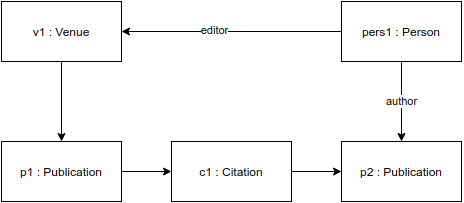
\includegraphics[width=9cm]{images/cite_work_editorial_board.drawio.png}
\caption{Instance model of citation of work of member from editorial board}
\label{fig:cweb}
\end{figure}

% ------------------------------------------------------------------------------
\paragraph{Attack} When this situation is being enforced (malicious intent), it 
becomes attack (e.g. the member says: "cite me, or your work will not be 
published"). The person of interest benefits from this situation; he will be
cited more, which impacts his metrics (e.g. H-Index). The question is how this
enforcement impacts the publication model so we are able to detect this.

% ------------------------------------------------------------------------------
\paragraph{Model impact}
The impact this attack has on the publication model is on the objects Venue, 
Person (with the role editor) and the relationship between. This relationship is
the fact that a person works for a venue. In this relationship, citations occur;
while a person works for a venue his work is being cited. In case of an attack; 
we see more citations than usual. The metric we need from this 
relationship is the number of citations: \textit{number\_of\_cites}. But we need
to take the time into account; if a person works for a venue for a long time 
(multiple incollection or inproceedings are published), it is to be expected the
number of cites while being a member is high. Because of this; we also need the 
number of incollection and inproceedings: \textit{number\_of\_issues}.
These metrics can be used for comparison by calculating the `normal' and the 
deviation of all members. This `normal' can be calculated over the venue the 
editor is working for, or all venues. This comparison makes it possible to 
identify interesting editors in comparison with his peers.

\begin{figure}[H]
\centering
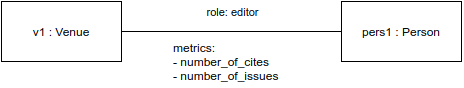
\includegraphics[width=9cm]{images/cite_work_editorial_boardmodel_impact.drawio.png}
\caption{Metrics needed for detection on publication model}
\label{fig:cwebimpact}
\end{figure}

% ------------------------------------------------------------------------------
\paragraph{Benign alternatives}
The described impact on the publication model can also have other benign reason 
to occur. The detection strategy is not foolproof. We need to take into account 
that a person is such an excellent contributor, it is logical he is being cited
far more that his peers.

% ==============================================================================
\section{Implementation}
% ==============================================================================
In this section we elaborate on the implementation of the flow to acquire and
integrate the data.

\subsection{Functional overview}

The focus of this case study are people on a position with influence.
People with influence can be found at top conferences and journals.
Therefore, the primary selection criteria are top conferences and journals.
These conferences are the input for the proceedings we need to collect. From 
these proceedings we need to get the articles published in the proceedings and
the PC Members involved. From the articles, we need to get the citations.
In Figure~\ref{fig:functional_overview} we draw this overview. The arrows mean
that, in case of the left arrow, the top conferences are input to get the 
proceedings (meaning only proceedings of the top conferences).

\begin{figure}[H]
    \centering
    \includegraphics[width=\textwidth]{images/case_study_1/implementation/functional_overview.png}
    \caption{Functional overview}
    \label{fig:functional_overview}
\end{figure}

From this functional overview of the situation we zoom into the implementation
for acquisition and interpretation.

\paragraph{A word about notation}
In this (and the other case studies') implementation chapter we draw elements to
represent applications and its inputs and outputs. See Figure~\ref{fig:notation}
for the notations used. 
The left box represents an application. The text in this box means that
the application can be found in the final repository\footnote{On GitHub
\url{https://github.com/woudw/IM9906}} in the directory `solution/subdir1/subdir2'.
The name of the (in this case Python script) is called `app.py'. In case of a .Net 
application, the text is `.net' and next line the directory of the application.
The parallelogram in the middle represents a relational storage in the database (table or 
view). The name on top is the schema name, the name under the schema name is the name 
of the table or view.
On the right we draw a cube which represents disk storage. The text between brackets
is the type of files stored.

\begin{figure}[H]
    \centering
    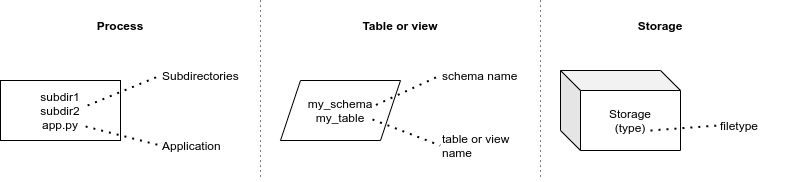
\includegraphics[width=\textwidth]{images/case_study_1/implementation/notation.png}
    \caption{Notation usage (left: application, middle: table or view, right: storage)}
    \label{fig:notation}
\end{figure}



% In this section we will elaborate which data we need and how we get that data.
% The flow from conference to proceedings is shown in
% Figure~\ref{fig:data_integration_core_dblp_api}. In the next subsections we 
% describe the process steps and datasets of this flow in more detail.

% \begin{figure}[H]
%     \centering
%     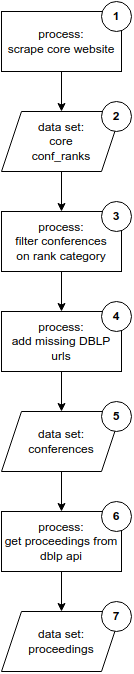
\includegraphics[width=3cm]{images/data_integration/core_dblp_api.png}
%     \caption{Gathering proceedings. The parallelogram are 
%     (intermediate) datasets and the rectangles are process steps.}
%     \label{fig:data_integration_core_dblp_api}
% \end{figure}

% ==============================================================================
\subsection{Top conferences}
The focus of this case study is people on a position with influence.
People with influence can be found at top conferences and journals.
Therefore, the primary selection criteria are top conferences and journals.
For our study, which focuses on computer science, we get the top conferences 
and journals from The Computing Research and Education Association of 
Australasia (core)\footnote{\url{https://www.core.edu.au/}}.
Core scores conferences with the following
ranking\footnote{\url{https://www.core.edu.au/conference-portal}}:
\begin{description}
    \item[A*] Flagship conference
    \item[A] Excellent conference
    \item[B] Good to very good conference
    \item[C] Other ranked conferences with minimum standards
\end{description}
Besides these four, they also have 'Australasian', 'Unranked', 'National', and 
'Regional', which is not of interest for our purpose.
Based on their ranking, we select the conferences for our 
research with a ranking of B or higher.
The CORE website provides an export functionality for acquiring data. However, 
for integration purposes, this is not sufficient; the export misses the link to 
the \dblp{} conference, which is available on their website. For that reason, we 
built a web scraper.

\subsubsection{CORE Scraper}
The scraper should be able to get the necessary information for our case 
study.
This tool does not depend on any input; it scrapes all data of the website.
In Figure~\ref{fig:functional_overview_top_conferences} we position this tool as 
implementation to
fulfill the functionality to get the top conferences. As shown, this tool has two
output tables: one for conferences and one for journals.

\begin{figure}[H]
    \centering
    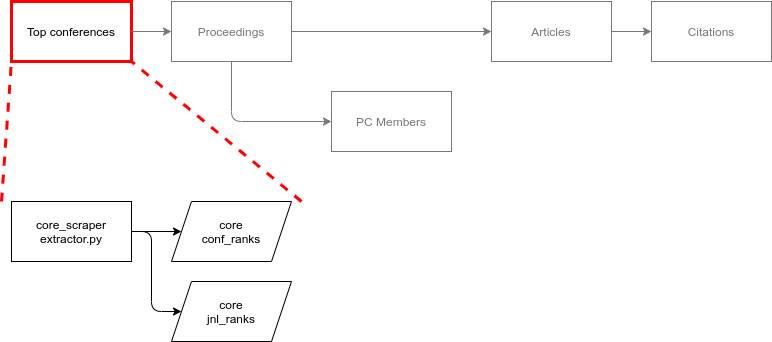
\includegraphics[width=\textwidth]{images/case_study_1/implementation/functional_overview_top_conference.png}
    \caption{Top conferences implementation}
    \label{fig:functional_overview_top_conferences}
\end{figure}

This tool does not store the data to disk before interpretation. The reason is 
that the data is represented in an HTML table (which is highly structured) and 
therefore can be directly inserted in the database.
The output of this scraper is not sufficient to acquire the proceeding information. 
Two steps need to be added:
\begin{itemize}
    \item The dataset misses 17 \dblp{} links, we add these by hand.
    \item We need to filter the conferences on the ranking.
\end{itemize}
These steps are implemented in dbt (Section~\ref{gen_impl:dbt}).

% ==============================================================================
\subsection{Proceedings}
With the selection criteria in place, we get the proceedings of the 
conferences from \dblp{}. \dblp{} provides the option to download the complete 
data dump from their website (described in Chapter~\ref{chp:data}). 
Unfortunately, conferences are not part of this dump. But, with the API of 
\dblp{} we are able to get the proceedings based on the searchterm from the 
\dblp{} url of CORE. Therefore, we built a tool to load this data from the 
\api{} in the database.
\subsubsection{DBLP API extractor}
In Figure~\ref{fig:functional_overview_proceedings} we position this \api{} 
extractor in the functional landscape.

\begin{figure}[H]
    \centering
    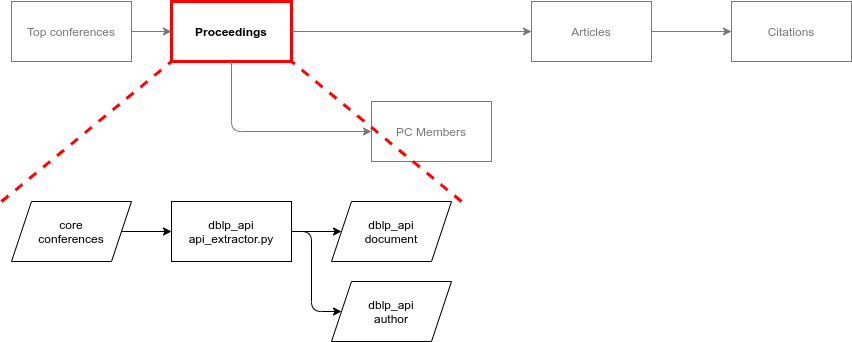
\includegraphics[width=13cm]{images/case_study_1/implementation/functional_overview_proceedings.png}
    \caption{Proceedings implementation}
    \label{fig:functional_overview_proceedings}
\end{figure}

As shown in Figure~\ref{fig:functional_overview_proceedings} the input is the
table core.conferences. This table is the output of the core scraper with the 
additional steps.
For every DBLP key in this conference set, we request all proceedings.

\begin{wrapfigure}{r}{0.5\textwidth}
    \centering
    \begin{tabular}{ lr }
        \toprule
        Publisher & \#proceedings \\
        \midrule
        Springer              & 4,751 \\
        ACM                   & 4,115 \\
        IEEE Computer Society & 2,422 \\
        IEEE                  & 1,210 \\
        \bottomrule
    \end{tabular}
    \caption{Publishers with $>$1,000 proceedings}
    \label{tbl:publisher-proceeding-count}
    % \vspace{-20pt}
    
\end{wrapfigure}

The output of this application are two tables: document and author. We focus on
document, which are the actual proceedings (author are the editors).
% ==============================================================================
In Figure~\ref{tbl:publisher-proceeding-count} we show the publishers with 
more than 1,000 proceedings.

% \begin{table}[h]
%     \caption{Publishers with $>$1,000 proceedings}
%     \begin{tabular}{ lr }
%         \toprule
%         Publisher & \#proceedings \\
%         \midrule
%         Springer              & 4,751 \\
%         ACM                   & 4,115 \\
%         IEEE Computer Society & 2,422 \\
%         IEEE                  & 1,210 \\
%         \bottomrule
%     \end{tabular}
%     \label{tbl:publisher-proceeding-count}
% \end{table}
For this case study we want to use the biggest source, which is Springer. 
Springer publishes their proceedings under the Lecture 
Notes of Computer Science (LNCS). The resulting set contains 4,467 unique 
proceedings (the DBLP API search function sometimes returns double results).

% ==============================================================================
% \subsection{Acquisition of the PC Members}
On the site of a \lncs{} proceeding, a front matter document is available for
download. A front matter document contains information about the proceeding,
including people involved in that specific conference; e.g. steering committee,
reviewers and, important for our case, the PC members.

The data acquired from the \dblp{} \api{} contains the \doi{} link to 
the proceeding on \lncs{} (for 1 document this misses, we added it manually). 
With this anchor we can start acquiring the necessary data, including the 
download link to the front matter document.

% ==============================================================================
\subsection{Proceeding information, articles and authors}
\label{subsec:springer_website}
To get the data from \lncs{} we built a web scraper. In 
Figure~\ref{fig:functional_overview_articles} we position this scraper in the 
functional landscape.

\begin{figure}[H]
    \centering
    \includegraphics[width=13cm]{images/case_study_1/implementation/functional_overview_articles.png}
    \caption{LNCS web scraper implementation}
    \label{fig:functional_overview_articles}
\end{figure}

The input for this web scraper are the \doi{} links from the \dblp{} \api{}.
The output are six tables: books (proceeding), chapters (article), editors and 
authors and their affiliation. See Figure~\ref{fig:lncs_scraper_datamodel} (page 
\pageref{fig:lncs_scraper_datamodel}) for a graphic representation of the 
entities and their relations. The relationships are 1 to many.
The book table is the actual proceeding. A proceeding is edited by an editor. 
A proceeding contains multiple chapters (\lncs{} terminology for article). A
chapter is written by one or multiple authors. The authors and editors may 
have one or many affiliations (e.g. universities, institutes, companies).

\begin{figure}[ht]
    \centering
    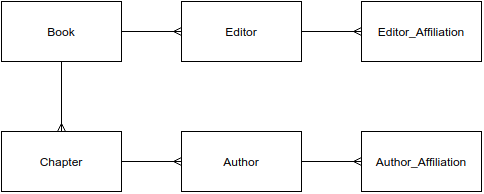
\includegraphics[width=11cm]{images/lncs_scraper_datamodel.drawio.png}
    \caption{Datamodel of the output of the \lncs{} scraper}
    \label{fig:lncs_scraper_datamodel}
\end{figure}

The output of this application is not stored to disk, but directly to the 
database. The reason is
that we need to interpret the proceeding page to get the article links; and while
we are interpreting the page, we interpret the other information as well. Also,
the data in the HTML page is mostly key-value based. As an example we show a 
piece of HTML of a proceeding page in Listing~\ref{lst:lncs_proceeding}.
This listing is a list (\verb|<ul>| tag) of items (\verb|<li>| tag). Every 
item has a span with classname ending in `title' 
(the key) and a span with a classname ending in `value'. Because of this 
standardization used
on the page, we can loop through the items and scrape all data. 
Combined with the automatic adjustment of the database table (see
Section~\ref{gen_impl:abstract_database}) we can add all these key-value pairs
to a dictionary and store them in the database.

\lstset{language=HTML}
\begin{lstlisting}[
    caption={Example HTML LNCS proceeding},
    label={lst:lncs_proceeding},
    numbers=left]
<ul class="bibliographic-information__list--inline">
  <li class="bibliographic-information__item">
    <span class="bibliographic-information__title">Book Title</span>
    <span
      class="bibliographic-information__value u-overflow-wrap"
      id="title">Mastering Scale and Complexity in
      Software Reuse</span>
  </li>
  <li class="bibliographic-information__item">
    <span class="bibliographic-information__title">Book Subtitle</span>
    <span
      class="bibliographic-information__value u-overflow-wrap"
      id="sub-title">16th International Conference on
      Software Reuse, ICSR 2017, Salvador, Brazil, May
      29-31, 2017, Proceedings</span>
  </li>
</ul>
\end{lstlisting}

The reason we also acquire the chapters is to get the relation between a book
and the articles it contains. To keep our main goal clear: we need to get the
people involved, so while we are scraping the articles, we can scrape the
authors (and their affiliations) just as well.
The most important entities we gather from \lncs{} are the books (proceedings), 
chapters (articles) and authors. The editors and their affiliation are not 
important for this case study. 
All chapters we scraped contain a \doi{} as attribute. 
By scraping the books we also get the link to the front matter PDF which can be 
used to download the front matter, which contains the PC Members.

% ==============================================================================
\subsection{PC Members}
\label{sec:front_matter_parsing}
Acquiring the PC Members is a two-step process. First we need to download the
PDF documents. The input are the URL's to the front matter. These are available
as attribute of the book (proceeding) object from the previous step. For this we
created a download tool which stores the data on disk. As name of the stored 
PDF we use the \dblp{} name of the proceeding so we are able to relate the PDF 
document to a proceeding.
After downloading the front matter documents, we need to parse the documents to
get the required information.
An overview how these two applications fit in the landscape is shown in
Figure~\ref{fig:functional_overview_pc_members}. After the figure, we will dive in
the details of the PDF parser and explain the tables shown as output (the red lines
are for visual distinction, they have no functional meaning).

\begin{figure}[ht]
    \centering
    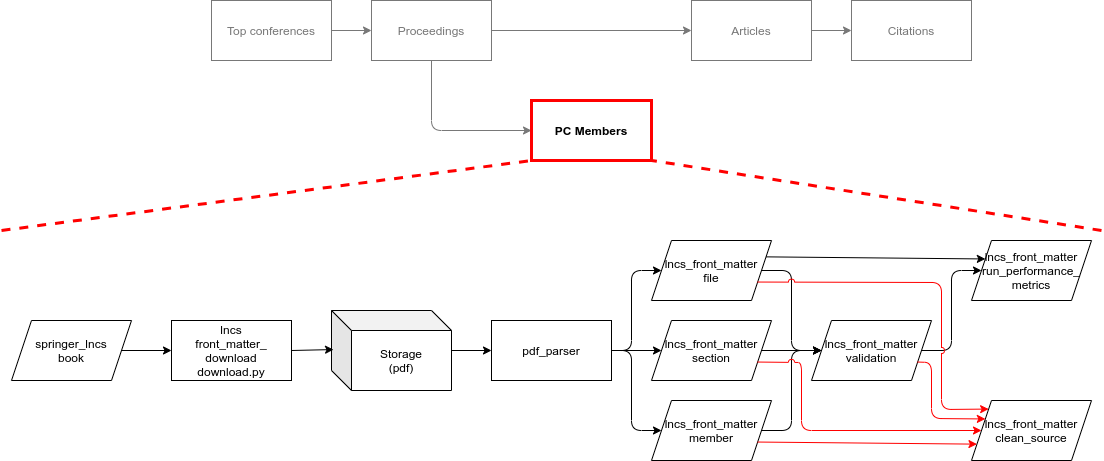
\includegraphics[width=\textwidth]{images/case_study_1/implementation/functional_overview_pc_members.png}
    \caption{Acquisition of PC Members implementation}
    \label{fig:functional_overview_pc_members}
\end{figure}

\subsubsection{Acquisition of information from the front matter documents}
In Section~\ref{gen_impl:pdf_scraping} we described the generic parsing of PDF
documents to textobjects which can be used for interpretation; converting 
content to information. Currently we have 4,370 Front Matter documents. To get
the information from these documents we built a prototype of a parser.

% ==============================================================================
\paragraph{Building a document tree}
\label{sec:lncs_parser_doc_tree}
By using the properties textsize and bold properties of the textobjects we are 
able to identify headers in the document which we need to build an hierarchical 
structure of the document. In most front matter documents there is an
organization header, with subheaders containing the role of the people.
The textsize is also used to identify content; these are textobjects with the
same size as the size which occurs most in the document. Sometimes documents
contain a footer or header with a smaller textsize as the content. By only using
textobjects with the size as the content, we ignore these footers and headers.

To be able to work with the document structure, we parse this hierarchical
structure in a tree datastructure. The objects we store in this tree are
Sections. These contain the textlines and the header as title of the section. 
In Figure~\ref{fig:front_matter_organisation_section} an organization part of 
a front matter document is shown. The format of this part makes clear that we 
need properties as text size and bold identification to identify headers. 

%%\parbox[H]{\textwidth}{
\begin{figure}[ht]
    \centering
    \fbox{\includegraphics[width=.7\textwidth]{images/front_matter/organisation_sections.PNG}}
    \caption{Organisation part in a front matter}
    \label{fig:front_matter_organisation_section}
\end{figure}


In
Listing~\ref{lst:document_tree} a textual representation of a part of
Figure~\ref{fig:front_matter_organisation_section} is shown.
The most important for our purpose is the section called 'Organization' with
the underlaying sections 'Steering Committee', 'General Chairs', 'Program Chair'
and 'Workshop Chairs', as these are the roles of people involved in this
proceeding. From the entire document tree, we can easily find the section that contains the
organisation and all sections underneath.

\begin{minipage}{\linewidth}
\begin{lstlisting}[
    caption={Representation of the organisation part},
    captionpos=b,
    label={lst:document_tree}
    ]
...
- - - {"section":{"title":"Organization","# lines":8}}
- - - - {"section":{"title":"Steering Committee","# lines":7}}
- - - - {"section":{"title":"General Chairs","# lines":7}}
- - - - {"section":{"title":"Program Chairs","# lines":7}}
- - - - {"section":{"title":"Workshop Chairs","# lines":8}}
\end{lstlisting}
\end{minipage}

% ==============================================================================
\paragraph{Processing a section}
A section is a textpart of the document. In 
Figure~\ref{fig:front_matter_section} an example is shown. In this example, the
role of the member is the title (Steering Committee).
\begin{figure}[ht]
    \centering
    
\includegraphics[width=12cm]{images/front_matter/section.png}
    \caption{Section in the Front Matter}
    \label{fig:front_matter_section}
\end{figure}
The text in a section with people involved in the proceeding, has a grid
structure. A visual representation of a grid laid on top of 
Figure~\ref{fig:front_matter_section} is shown in 
Figure~\ref{fig:front_matter_section_grid}. 
% ==============================================================================
\begin{figure}[H]
    \centering
    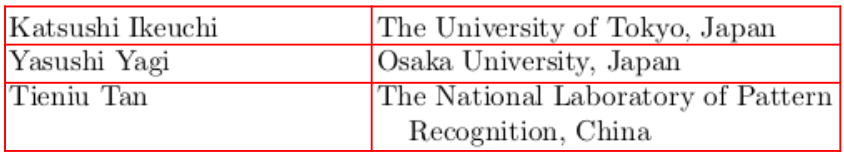
\includegraphics[width=12cm]{images/front_matter/section_table.png}
    \caption{Section in the Front Matter}
    \label{fig:front_matter_section_grid}
\end{figure}
% ==============================================================================
Because of this structure, we use a grid as data structure to put the data from 
the raw lines into. In Listing~\ref{lst:grid_representation} we show the 
parsed section in a grid representation from the logs files. The challenge in
this part is to merge lines into one line. This process is done by dedicated
section-to-grid object. Separating this process from the process of building a
tree, improves testability.

\begin{lstlisting}[
    caption={Representation of the grid (captured from the application logs)},
    captionpos=b,
    label={lst:grid_representation}
    ]
+------------------+-------------------------------------------------------+
| Katsushi Ikeuchi | The University of Tokyo, Japan                        |
+------------------+-------------------------------------------------------+
| Yasushi Yagi     | Osaka University, Japan                               |
+------------------+-------------------------------------------------------+
| Tieniu Tan       | The National Laboratory of Pattern Recognition, China |
+------------------+-------------------------------------------------------+
\end{lstlisting}

This grid structure gives us some possibilities, e.g. to get statistics of a
column, which we are going to need to choose the correct parser to transform
this text into information.

\paragraph{Getting information from a grid}
\label{subsec:front_matter_grid_information}
To get information from a grid we need to parse the text in the grid. For 
this we define a parser interface. The implementation of this interface 
depends on the structure of the grid (e.g. the number of columns) and the 
content (e.g. is it an affiliation or a name).

Determining which implementation of the parser is needed, is done by a 
\verb|GridParserFactory| which uses the statistics and format of a grid. The 
properties collected from the grid to choose the correct parses are:
\begin{itemize}
    \item \emph{Number of textparts}: The total number of cells that are filled
    in the grid.
    \item \emph{Number of columns}: The number of columns that the grid
    contains. Most sections contain two columns, but this is certainly not the
    case for all sections.
    \item \emph{Affiliation ratio}: The ratio of textparts that contain keywords
    for an affiliation (e.g. "universi"). This is calculated for every 
    column and for odd, even and all rows.
    \item \emph{Comma ratio}: Same as affiliation ratio, but for commas. Can
    also be used to identify affiliations. However, names also contain 
    commas if the format is lastname, firstname.
\end{itemize}

The affiliation ratio and comma ratio is calculated for odd, even and all
rows. The reason is that sometimes the affiliation is presented under the
name of the member. In Listing~\ref{lst:front_matter_grid_info} we show 
some statistics for identifying affiliations.

\begin{lstlisting}[caption={Some derived information from the grid},captionpos=b,label={lst:front_matter_grid_info}]
numberOfColumns:	2
affiliationRatios:
	{"columnNumber":0,"rows":"ALL","ratio":0.0}
	{"columnNumber":0,"rows":"ODD","ratio":0.0}
	{"columnNumber":0,"rows":"EVEN","ratio":0.0}
	{"columnNumber":1,"rows":"ALL","ratio":0.6666666666666666}
	{"columnNumber":1,"rows":"ODD","ratio":0.5}
	{"columnNumber":1,"rows":"EVEN","ratio":1.0}
\end{lstlisting}

With this information the \verb|GridParserFactory| can choose the appropriate 
implementation of the parser to interpret the data correctly and 
convert the grid into information (members and affiliations). 
%
For example, Listing~\ref{lst:front_matter_grid_info} shows us that 
the ratio of affiliation keywords in the second column (0-based) is 
above a certain threshold and the section consists of two columns, the software 
chooses a \verb|Two_Name_Affiliation| parser which means two columns, first column is a 
name, second column is the affiliation.
%
The resulting objects are shown in 
Listing~\ref{lst:front_matter_resulting_information}.
\begin{lstlisting}[
    caption={Resulting information (from the logs, reformatted for readability)},
    captionpos=b,
    label={lst:front_matter_resulting_information}
]
{
    "name":"Katsushi Ikeuchi",
    "affiliation":"The University of Tokyo, Japan",
    "role":"Steering Committee"
}
{
    "name":"Yasushi Yagi",
    "affiliation":"Osaka University, Japan",
    "role":"Steering Committee"
}
{
    "name":"Tieniu Tan",
    "affiliation":"The National Laboratory of Pattern Recognition, China",
    "role":"Steering Committee"
}
\end{lstlisting}


% ==============================================================================
\subsubsection{Output}
This process to parse PDF files to usable information creates the 
following data:
\begin{itemize}
    \item \emph{Information dataset}: The process outputs the members (name
        and affiliation), the role and the document this information was read 
        from.
    \item \emph{Metadata}: Besides this information, the statistics described in~`\nameref{subsec:front_matter_grid_information}' and the used parser 
        implementation is also added. We use this to validate the results; we will come back to this in~`\nameref{sec:front_matter_validation}'.
    \item \emph{Logging}: For every PDF the application parses, a log file is created.
        The purpose is error-detection and the possibility to quickly gather 
        information to extend the software and create the tests; iterative 
        logging-based development.
\end{itemize}


\paragraph{Iterative logging-based development process}
For every PDF that the program processes, it keeps a separate logfile. This
gives us the ability to investigate why the program was unable to process some
files or sections. Missing parser for example can be detected using this
mechanism in combination with the data in the section table in the database.

For every file the logfile shows the document tree (e.g.
Listing~\ref{lst:document_tree}). If sections are found, the logfile shows for
every section:
\begin{itemize}
    \item \emph{Textlines}: All the lines that are in this section.
    \item \emph{Grid}: The derived grid from the textlines (e.g.         Listing~\ref{lst:grid_representation}).
    \item \emph{Members}: The members that are extracted from the section.
\end{itemize}
Having this information gives us the possibility to 
investigate in detail why data can not be interpreted and easily build new 
functionality (e.g. new parser implementations) and add unit tests for this 
functionality.

\subsubsection{Validation}
\label{sec:front_matter_validation}
Currently 4,370 front matter documents are available. How are we able to tell 
something about the quality of the program without manually going through the 
results?

For every section we gather some metrics (e.g. number of lines read, number of 
lines merged, chosen parser). This data is stored in the output dataset (file, 
section, member) shown in
Figure~\ref{fig:functional_overview_pc_members} on the right side.
With these metrics, depending 
on the parser we can see if the number of extracted members is correct. This 
data is stored in the validation table.
For example, the parser Two\_Role\_NameAff contains two columns: first with a name
and second with the affiliation. We can measure if the number of resulting 
members is equal to the number of non-empty lines in the section minus the number 
of merged lines. If it is, we can use the extracted members with confidence; 
the data is read correctly.

Based on these 4 datasets (file, section, member and validation) we can create
2 tables: one table with performance statistics of the run (e.g. how many
sections are corrected interpreted) and a dataset which contains 'cleaned'
data. This cleaned data transforms the different roles to a standard set of 
roles and only contains validated data; this makes sure this use case only uses
validated data. All these transformations are done using SQL (dbt,
Section~\ref{gen_impl:dbt}).

\paragraph{Current state}
In Figure~\ref{fig:front_matter_result} we show a tree with the file counts.
The input for this tree is the performance statistics table described 
previously. From the 4,370 files we were unable to process 1,237 files of which
1,119 because the software was unable to find the organization header. It may be
useful for improvement of the software to tackle this issue first.
Of the correct processed files, 2,223 contained interesting sections. These are
section with the role 'program committee'. Among these interesting section, 2,711
across 2,055 files are validated with the above described method and can be used
during analysis. This `good' path is shown in red.

\begin{figure}[H]
    \centering
    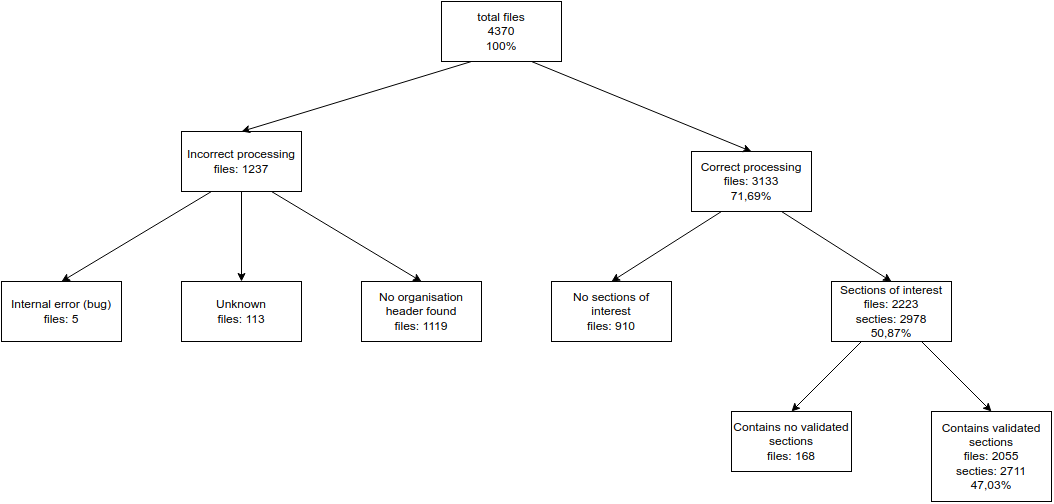
\includegraphics[width=17cm]{images/lncs_front_matter_result.png}
    \caption{Current results}
    \label{fig:front_matter_result}
\end{figure}

% ==============================================================================
\subsection{Citations}
Sources to acquire citation information are discussed in
Section~\ref{sec:data_public_datasets}. All chapters (articles) we scraped 
from the website contain a \doi{} as attribute. Therefore, the source we use
is OpenCitations (this source is \doi{}-based).
%
The data of OpenCitations can be downloaded in CSV format or requested by an
API. An experiment using the API resulted in a very slow process of acquiring
the data. Therefore, we choose to download the data. This data is stored on disk
storage. However, this dataset contains a lot of data separated over multiple 
files. Not all data is required; only citations of articles from the \lncs{} 
proceedings. 
%
To process the CSV files from OpenCitations for only the articles of \lncs{}, we 
need a software component. In Figure~\ref{fig:functional_overview_citations}
(page \pageref{fig:functional_overview_citations}) we
place this application in the functional landscape.
The input for this application are the stored CSV files and the chapter table 
acquired from scraping the \lncs{} website for the \doi{} attribute.

\begin{figure}[ht]
    \centering
    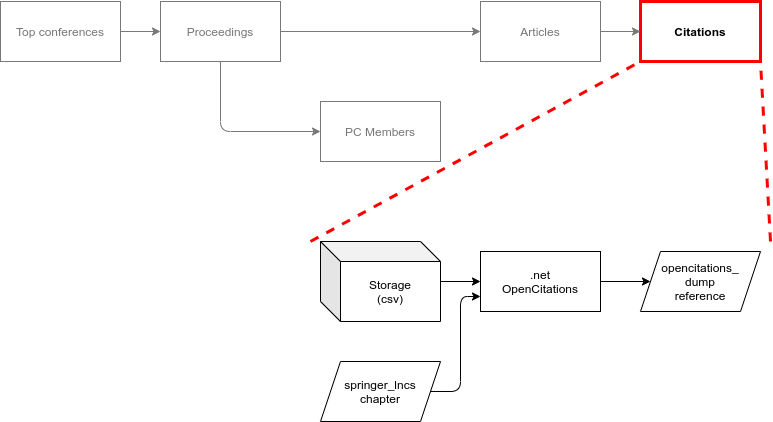
\includegraphics[width=13cm]{images/case_study_1/implementation/functional_overview_citations.png}
    \caption{Acquisition of citations.}
    \label{fig:functional_overview_citations}
\end{figure}

The tool iterates through the files (every line is
one citation) and stores the citation if the `from' \doi{} is in the set of 
articles. However, because of the amount of files and data, this tool will 
benefit from some performance improvements:
\begin{itemize}
    \item \emph{Parallel processing}: this tool is multi threaded and processes
    the amount of files in parallel same as the amount of CPU's available.
    \item \emph{Caching of the article \doi{}'s}: because the tool needs to
    check if the `from' \doi{} is in the list of article \doi{}'s, we need to
    cache this list. We tried three options: a list of strings, an arrray of
    strings and a HashMap. The HashMap was significantly faster.
\end{itemize}

The output of this application is one table with citations from an article in 
the \lncs{} proceedings to other \doi{}'s.


% ==============================================================================
\subsection{Formalising the integration dataset}
In this section we explain how we integrate the data we collected from the 
sources.

% ==============================================================================

% ==============================================================================

In the resulting dataset we combine the \dblp{} dump (see Section~\ref{sec:data:dblp}) 
with the data acquired from the previous section.
In Figure~\ref{fig:members_integration_citation} we show the sources and their 
relationships to create this dataset. Explanation will follow after the figure.
\begin{figure}[ht]
    \centering
    \includegraphics[width=16cm]{images/data_integration/members/members_integration_citation.png}
    \caption{Formalising the citing dataset by joining sets based on keys}
    \label{fig:members_integration_citation}
\end{figure}

We will describe this set clockwise starting in the top left. The keys and
foreign keys within a source (\dblp{} dump, Springer website) are not described
here.
The front matter \emph{member} (upper left) is the result of applying a filter
to use validated data. Because we use the \textit{\dblp{} key} in the name of
the PDF file, we can join this set with the proceeding (\emph{book}) of the
Springer website.
%
The Springer website part (top middle) is described in 
Subsection~\ref{subsec:springer_website}. The interested entities for this set
are the book and the \emph{chapter}s (articles) in this proceeding. 
%
From the chapter we get the \emph{reference} by the \textit{\doi{}} attribute 
(chapter \doi{} to reference `from \doi{}'). From this reference set we get the 
referenced articles from the \dblp{} dump by using the `to \doi{}' to the 
\emph{\doi{}} in \dblp{} dump.
%
Within the \dblp{} dump we have the names of the authors
of this referenced article in the \emph{person} set, which we can eventually
use to go back to the \emph{member} name.

Two choices are made by composing this set:
\begin{itemize}
    \item The relationship on the \textit{name} from \emph{person} to 
        \emph{member} is optimistic; the join is on the raw name. 
        However, because we use \dblp{} we match against possible multiple names
        of the author (see Section~\ref{sec:integrability_people}).
    \item Because we use OpenCitation, we only refer to articles in \dblp{}
        which contain a \doi{}. Another consequence is that we rely on the
        completeness of  OpenCitation, but this is an issue with every source we
        use.
\end{itemize}

% ==============================================================================

The implementation of the flow is added in 
Appendix~\ref{appendix:dataset_pcmember_citation}.

\subsubsection{Added value of these datasets}
By having these datasets we can calculate citation metrics for 
PC members and 
compare them with their peers, which may be in the same proceeding or across 
proceedings, depending on the scope of the peers.

% ==============================================================================
\section{Analysis and validation}
\label{sec:cs1_analysis}

In this paragraph we validate if acquiring the data with the focus on PC member
citations actually help to identify cases which can be further manually 
investigated.
From the defined dataset we have the for every member the \emph{count the
members' work is cited in the proceeding he was a member of}. 
As analysis we focus on citations from Symposium on String Processing and
Information Retrieval (SPIRE) as an example. The dataset 
contains observations of 483 PC members over 17 years (2003 - 2020).
In Figure~\ref{fig:citation_frequency} we show the frequency of citations. We notice
a large number of zero citations, which means that members during an activity 
(being PC member for a certain proceeding) are not being cited.

\begin{figure}[ht]
    \centering
    \includegraphics[width=\textwidth]{images/case_study_1/citation_frequency.png}
    \caption{Frequency of citation count}
    \label{fig:citation_frequency}
\end{figure}

In this phase we need to set the threshold to define an outlier. Eventually
this should be a decision made by domain experts of the publication process.
For our purpose and as an example
analysis we decide to place a threshold at 10 citations; every activity with
more than 10 citations is marked as an outlier.

In Figure~\ref{fig:analysis_few} we plotted a few PC member activities. 
Every dot is a member for a certain year of the publication.
The X-axis is ordered by member and year. E.g. we see that 
Member A has 3 citations for the 2018 proceeding. The Y-axis is the number of 
citations. The red dot in the 
top-right indicates that an activity is an outlier. By plotting the data 
this way, we can quickly
see clusters of outliers, which may indicate members that continuously have 
more citations than their peers.

\begin{figure}[H]
    \centering
    \includegraphics[width=16cm]{images/case_study_1/analysis_few_members.png}
    \caption{Example of citation data from Symposium on String Processing and 
    Information Retrieval (SPIRE). (Red lines added for clarity)}
    \label{fig:analysis_few}
\end{figure}

In Figure~\ref{fig:analysis_members} we plotted PC member activities for all PC 
members in SPIRE. The red dots are identified as outliers. One can clearly
identify a cluster (circled by a red dotted-line) which is the same PC member
with activities in multiple years (the name is known by the authors).

\begin{figure}[H]
    \centering
    \includegraphics[width=16cm]{images/case_study_1/analysis_total.png}
    \caption{How often each SPIRE PC member (1993-2020) was cited by each SPIRE where they were PC members.}
    \label{fig:analysis_members}
\end{figure}

% ==============================================================================
As validation we investigate if the outlier found in the analysis is correctly 
identified as an outlier. We can look at validation from a data acquisition
and integration perspective.

\paragraph{Data acquisition}
Validation of the front matter parsing is described in 
Section~\ref{sec:front_matter_validation}:~\nameref{sec:front_matter_validation}.
%
For other sources, we consider the datasets as given. These datasets are 
considered the building blocks for this research (as they are described in 
Chapter~\ref{chp:related_work}).
%
For the outliers found during analysis we manually verified that the data was 
correctly parsed from the PDF files. This was
indeed the case. We also noticed that this person was also related to other
conferences
for SPIRE, which were not correctly loaded because of a parse error.
%
The analysis is based on the whole population across all years. 
Our definition of an outliers can differ if we change the scope (e.g. `7' as 
threshold). However, as mentioned, this for a domain expert to decide.

\paragraph{Integration}
We took an optimistic approach in joining the different datasets together 
because of the limitation in the data described in Chapter~\ref{chp:data}. It
is therefore likely we miss some data. The effects of missing data could be:
\begin{itemize}
    \item Unmatched members in the authorset because the names differs;
    \item Too many authors mathed to a member because of the same name (for
    the outlier we found we verfied this was not the case);
    \item Unlinked referred papers because of the lack of DOI of the reffered 
    paper (the papers from LNCS do all have a DOI provided).
\end{itemize}

\section{Case study conclusion}
In this chapter we looked at the PC Members and how many times their work had
been referred in their proceedings. 
Despite the above described threads to the validity, we are able to identify 
outliers. From the 483 members involved in the Spire proceedings, we were able 
to identify 1 notable author. Depending on the threshold to be set by domain 
experts, this number may increase. Therefore, we can conclude that integrating 
data containing members of proceedings helps to direct manual effort to detect 
possible fraud.

% ==============================================================================
\chapter{Case study 2: Journal editors}
\label{chp:case2}
% ==============================================================================
In this chapter we focus on journal editors (editor-in-chief and the associate
editors) of ACM (Association for Computing
Machinery)\footnote{\url{https://dl.acm.org/}}; a publisher of journals in the
area of Computer Science. Just like in the previous case study, we will start
with a motivation and example of an attack, proceed with the data acquisition
and integration and conclude with an analysis of the data and validation of the
analysis.

% ============================================================================
\section{Motivation}
This case study focuses on journal editors, which are in position with great 
power. As previously shown in Figure~\ref{fig:c2013} (repeated in 
Figure~\ref{fig:c2013_2}), both roles are in a position power to make or break 
a publication and the career of an author.

\begin{figure}[H]
\centering
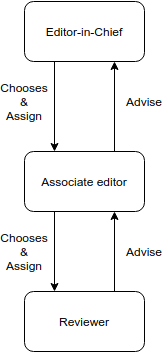
\includegraphics[width=3cm]{images/c2013.drawio.png}
\caption{Roles within the journal process (visual interpretation of description in~\cite{C2013})}
\label{fig:c2013_2}
\end{figure}

\newpage

\subsection{Interesting case: Member of the editorial board is (co-)author}
\label{interesting_case:member_editorial_board_is_coauthor}

In this case, publications in a venue are co-authored by a member of the 
editorial board, which means he is publishing his own work. A questionable 
case in this situation is
\mbox{Griffiths}\footnote{\url{http://deevybee.blogspot.com/2020/07/percent-by-most-prolific-author-score.html}}.
In Figure~\ref{fig:eia} we present an instance model of this situation.

\begin{wrapfigure}[17]{r}{0.3\textwidth}
    \centering
    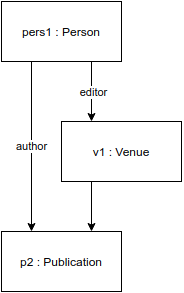
\includegraphics[width=0.3\textwidth]{images/editor_is_author.drawio.png}
    \caption{Instance model of the situation where the editor is \mbox{(co-)author} of the publication}
    \label{fig:eia}
\end{wrapfigure}

\paragraph{Attack}
We can imagine a situation in which the author is being forced to mention the 
person-of-interest as co-author; which is abuse of the power of the editor.

\paragraph{Model impact}
The impact on the publication model is between the person which is 
\mbox{editor} for a 
venue, and the venue itself. 
The number of publications he has in that venue while he works for that 
particular venue 
will increase. For detection we can measure this number of publications:
\textit{number\_of\_publications}. Also with the 
case described in 
Section~\ref{interesting_case:work_member_editorial_board_cited}, we need the 
number of issues.

% ------------------------------------------------------------------------------
\paragraph{Benign alternatives}
Besides possible ethical questions that can be raised, there may be a valid
reason for someone to publish in the venue he is editing. For example a person
is a 
specialist in his field and works at a venue which specializes in this 
specific subject. He has new work to publish but there is not another venue 
which captures this subject.

\subsection{Case study purpose}
\label{subsec:case2_purpose}
As with all case studies we try to prove that adding data not yet integrated in
known datasets and applying a group based outlier detection improves fraud
detection. In this case, the group of focus is the editorial board.
We need to compare members of this group. For comparison, we need to identify
the properties that make them different and may be indicating an attack on the
publication model.

As stated in the interesting case described in 
Section~\ref{interesting_case:member_editorial_board_is_coauthor}, a possible
attack if being forced to add a member of the editorial board as co-author. One
possible detection method is to see the ratio of unique authors the
person-of-interest published in the journal and outside the journal. If a member
publishes inside the journal with much more unique authors than outside the
journal, this may indicate this member forces the original author to make him
co-author. This case is based on the assumption that authors have their group of
peers they publish most of the articles with. In this case study, this is the
method we are going to apply.

% ==============================================================================
\section{Implementation}
In this case study our focus is the editorial board. Editor-in-chiefs, 
associate-editors and sometimes a list of reviewers (generic, not who reviewed 
what paper) are most of the time available on the publisher website of the 
specific venue. But this has two issues:
\begin{itemize}
    \item \emph{Machine readability}: These roles are not easy machine readable 
    through an interface. It is placed on the website for humans to read. 
    Although good technology exists to acquire data from a website, a minor 
    change to 
    the website can break this method and is therefore not a sustainable
    solution.
    \item \emph{Issue- and time awareness}: Only the current editorial board is 
    shown on the publisher website. This may be sufficient for guests of the 
    site, but for extending the datamodel with the editorial board with the 
    purpose of detecting fraud, this is not sufficient. In that case we need 
    to know who was editor for which issue. 
\end{itemize}
Not everything is lost however; most of the time the previous editorial 
boards are available in so-called mastheads or editorials of a certain 
issue. These 
mastheads can be downloaded as a PDF (as article of a journal). A formal 
investigation during the research preparation learned us that the format in 
which the editors are presented is not consistent (comparable with the 
front matter of the \lncs{} proceedings).

Theoretically, we can process the data as we did with the \lncs{} Front 
Matter. However, our intention is to prove the added value of additional 
publicly available data
by applying an outlier detection approach within the group of editorial 
board members. As we already gathered data from PDF's in Case study 1, 
we will not repeat this technical step (we already show that this is 
possible) and focus more on the functional added value of having 
editorial board members.

We choose ACM because ACM is a big publisher in the area of computer science
and they present the editorial members in a structured manner on their 
website for all journals. This makes acquiring the data in a automatic 
manner possible. To this this, we built a web scraper. In
Figure~\ref{fig:functional_overview_editors} we show that, to acquire the
editors (functional entity on top), we need to implement the presented flow.
Details of the implementation will follow after the Figure.

\begin{figure}[H]
    \centering
    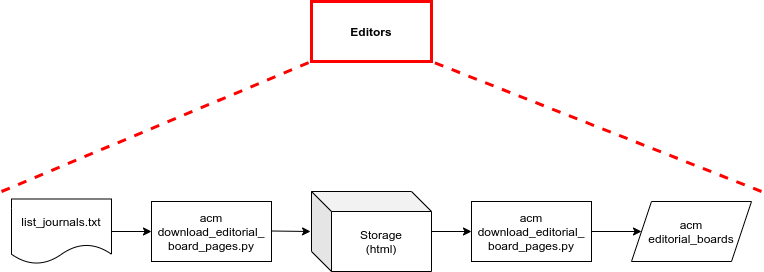
\includegraphics[width=13cm]{images/case_study_2/implementation/functional_overview_editors.png}
    \caption{Editors acquisition}
    \label{fig:functional_overview_editors}
\end{figure}

First we need to acquire the journals of ACM. Unfortunately, we were unable to
find such a list on the website of ACM. Luckily, we found another website with a
list of computer science journals of 
ACM\footnote{\url{http://oscar-lab.org/people/~jxuan/page/resource/acm-jour.htm}}.
We manually converted the table on this site to a textfile with urls; in
Figure~\ref{fig:functional_overview_editors} show as \verb|list_journals.txt|.
Given this list, we download the pages containing the editors using the
\verb|download_editorial_board_pages.py| and store the HTML files on disk. 
Not working links are ignored.
Figure~\ref{fig:acm_editorial_board} shows a screenshot from a part of the 
editorial board page of an ACM journal.

\begin{figure}[ht]
\centering
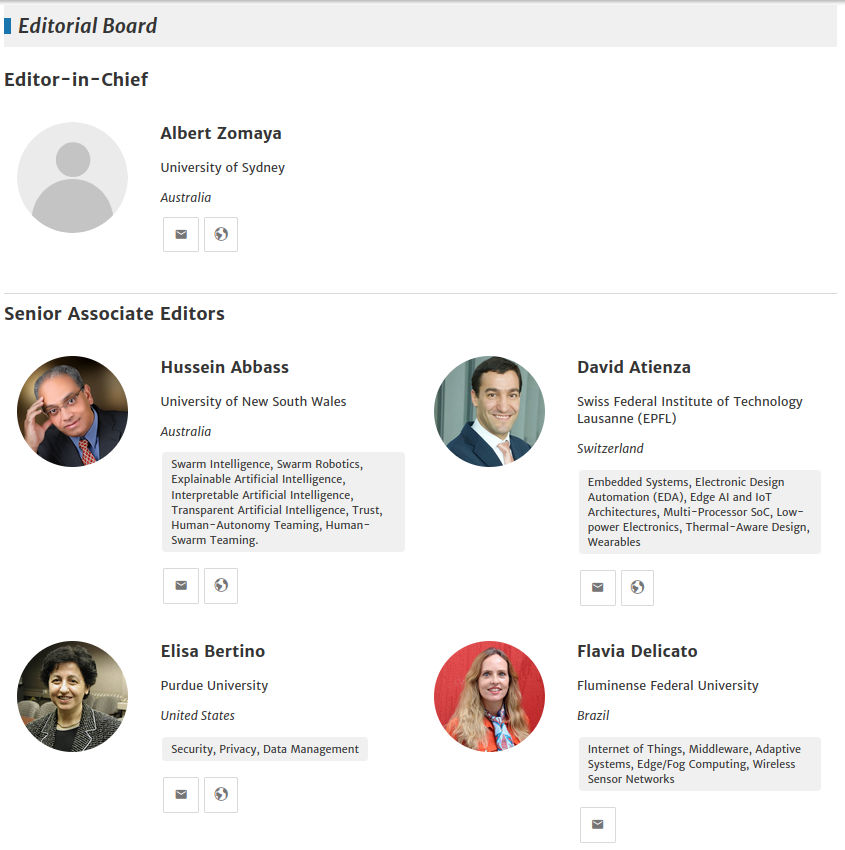
\includegraphics[width=11cm]{images/acm_editorial_board.png}
\caption{Page with editorial board from ACM (\url{https://dl.acm.org/journal/csur/editorial-board})}
\label{fig:acm_editorial_board}
\end{figure}

An editorial board page consists of `sections'. In the case of 
Figure~\ref{fig:acm_editorial_board}, the sections are `Editor-in-Chief'
and `Senior Associate Editors'.
These sections are defined by an HTML \verb|<h3>| 
tag with `section\_\_title' as class name. In case of the Senior 
Associate Editors, we can visually identify that the editors are placed 
in a grid of rows and columns. In the HTML these are represented as a
row (a \verb|<div>| with `row' as class) with columns (`col' as class).
However, the actual editor information is all located in a \verb|<div>| 
with `profile-meta' as class, so the `col' is not needed for parsing. 
This construction of the page defines the logic of the parsing 
application:
\begin{enumerate}
    \item Search for tags with class `section\_\_title' (use the content as role description);
    \item Under this section tag, collect all rows until another section tag
    is found, or the end of the document is reached;
    \item Within these rows, search profiles;
    \item Get information from these profiles.
\end{enumerate}

In Listing~\ref{lst:acm_profile_information} the HTML of profile information
is shown. All necessary information is in a \verb|<div>| with class 
`item-meta\_\_row' (except for the country). Unfortunately, this page does
not contain descriptive elements (e.g. `editor-name' as class values).
Therefore, we only can rely on tags like \verb|<h4>| to determine the name.
This is very error-prone, if the publisher decides the name should be in another 
tag (e.g. \verb|<h3>|) we are unable to acquire the name.

\newpage
\lstset{language=HTML}
\begin{lstlisting}[
    caption={HTML of profile information ACM (removed unnecessary parts for readability)},
    label={lst:acm_profile_information},
    numbers=left]
<div class="profile-meta">
  <div class="item-meta__info">
    <div class="item-meta-row">
       <h4 class="item-meta-row">Elisa Bertino</h4>
    </div>
    <div class="item-meta-row">
      <p>Purdue University</p>
    </div>
    <em>
      <span style="font-style: italic; font-size: 14px;">United States</span>
    </em>
  </div>
</div>
\end{lstlisting}

The resulted attributes we acquire from the people on these pages are: role,
name, affiliation, country and journal name.

% ==============================================================================
\subsection{Formalising the dataset}
As stated in Section~\ref{subsec:case2_purpose} we want to have the number of
unique co-author a member publishes inside and outside a journal. For this we
need the following entities:
\begin{itemize}
    \item Editors
    \item Articles written by these editors
    \item Co-authors of these articles
    \item The venue where these articles were published
\end{itemize}

We already acquired the editors from the ACM website. The other entities can be 
found in the \dblp{} dump. 
However, the venue is not straightforward in the dump of \dblp{}; it is 
encapsulated in the key of an article, see Listing~\ref{lst:dblp_object_key} 
as example.

\lstset{language=XML}
\begin{lstlisting}[caption={Example DBLP key},label={lst:dblp_object_key}]
journals/tomccap/Wang21
\end{lstlisting}

In case of the example, \verb|tomccap| is the abbreviation of the journal.
However, the name we get from ACM website is only the full name of a journal. In
this case `ACM Transactions on Multimedia Computing, Communications, and
Applications'. More interesting; this full title is also abbreviated as
\verb|tomm|; thus the relation between a journal name and abbreviation is not
1-on-1.

% ------------------------------------------------------------------------------
\subsubsection{Journal abbreviation lookup}
We need a dataset containing the relationship between the abbreviation and the
full journal name. Two sets were found:
\begin{itemize}
    \item \emph{Pages at Clarivate}: which are the maintainers of Web of
    Science. Unfortunately, the abbreviations used by \dblp{} were not found in
    this set.
    \item \emph{University of British Columbia}: also maintains a list. However,
    the abbreviations they use are different. E.g. in case of the example, their
    abbreviation is `ACM Trans. Multimedia Comput. Commun. Appl.'. \dblp{}
    also abbreviates journalnames this way, but the 
    abbreviations from this university are not found in \dblp{}.
\end{itemize}
The list of journals we want to scrape from ACM is limited: only 27. So
a manually built dataset is a valid solution. This is very achievable 
with help of the search functionality on the \dblp{} site. See 
Figure~\ref{fig:dblp_search_result} as example; the abbreviations used are shown
directly right to the name.
\begin{figure}[H]
\centering
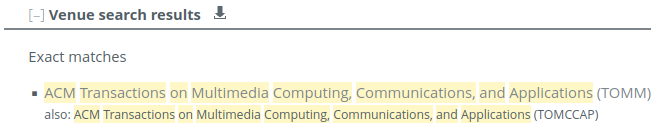
\includegraphics[width=11cm]{images/dblp_search_result.png}
\caption{DBLP search result (\url{https://dblp.org/search?q=ACM+Transactions+on+Multimedia+Computing\%2C+Communications\%2C+and+Applications}).}
\label{fig:dblp_search_result}
\end{figure}
% ------------------------------------------------------------------------------
\subsubsection{Integration model}
With the information from the previous section, we can now build the dataset to
perform our analysis upon. The dataset formulation is shown in 
Figure~\ref{fig:editors_integration_coauthor}. The explanation will follow 
after the image.
\begin{figure}[H]
    \centering
    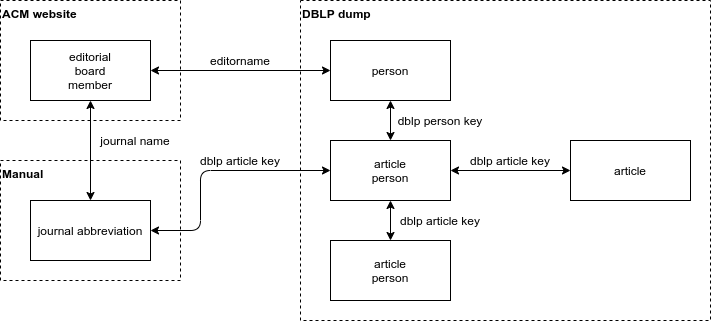
\includegraphics[width=\textwidth]{images/data_integration/editors/editor_integration_coauthor.png}
    \caption{Formalising the publishing dataset}
    \label{fig:editors_integration_coauthor}
\end{figure}
We start with the editors from the ACM website. By joining the editorname 
to the authorname in DBLP, we can get the unique DBLP name key (because of the 
issues with people covered in Section~\ref{sec:integrability_people}). With this 
key we can get all the articles written by the editor from the `article person'
table. By joining again with the `article person' table on the article key we 
can get the DBLP person keys for all co-authors.

To know if an article is published in the same journal the person-of-interest 
is member of, we need to identify if the journal from the ACM website is the 
same of the article published. In the previous section we elaborated on the 
issues involved here. By using a manual dataset as link table, we can identify
if the article is published in this particular journal. For this scenario we
extracted the journal abbreviation from the DBLP article key.
Additional information about the article can be achieved from the article table.

% ==============================================================================
\section{Analysis and validation}
% \outline{
% \begin{itemize}
%     \item Wat betekent de data?
%     \item Alleen laatste jaar want; alleen actieve editorial board
% \end{itemize}
% }

The properties of the editors we work with are \textit{Number of unique 
coauthors inside the journal} and \textit{Number of unique 
coauthors outside the journal}. From the dataset we removed publications the 
editor wrote himself. In the number of unique authors, the editor is excluded.
In Figure~\ref{fig:editors_in_out_journal} we plotted the editors.
On the X-Axis
the number of unique coauthors the editor has worked with inside the journal, on 
the Y-Axis the number of unique coauthors the editor has worked with outside the 
journal. 

For the purpose of this case study (described in 
Section~\ref{subsec:case2_purpose}) interesting cases should show up in the right 
bottom (high number of unique coauthors inside the journal, and low outside the 
journal).
To clearly show the ratio we draw a diagonal on \(x = y\). In area with the red 
background the number of coauthors inside the journal is higher than outside the 
journal.
The highlighted observations will be described after the figure.

\begin{wrapfigure}{r}{0.55\textwidth}
    \centering
    \includegraphics[width=0.40\textwidth]{images/case_study_2/in vs outside.png}
    \caption{Number of unique coauthors inside vs outside the journal per editor}
    \label{fig:editors_in_out_journal}
\end{wrapfigure}

\paragraph{Observation 1}
This editor worked with 15 unique authors on 15 publications inside the journal 
and 15 unique authors on 18 publications outside the journal.
This means with all coauthors, he publishes one article inside the journal,
which is the expected behaviour.
Outside the journal, we notice 2 authors he wrote more than one article with. 
But on a population of 15 coauthors, this is not remarkable.

\paragraph{Observation 2}
Observation 2 has almost twice the number of unique coauthors outside the 
journal. Although observation is far to the right, compared with the 
population, this would not the a priority case to investigate.

% ==============================================================================
\paragraph{Observation 3}
We highlight this editor because the number of unique coauthors 
inside the journal significantly exceeds the number of unique coauthors outside 
the journal. 
This editor worked with 16 unique authors on 5 publications inside the journal 
and 9 unique authors on 3 publications outside the journal. In the period under
investigation, there is no coauthor with whom this editor has published both
inside and outside the journal. However, if we extend  the period to include
2019, we find 3 scientists that have coauthored papers both within and outside
the journal. Further analysis shows that this editor only publishes once with
each of his colleagues, except one. Such behaviour is in line with the above
described fraud  -- though it should not be mistaken as evidence for it. Indeed,
this pattern holds for both coauthors within and outside the journal. The latter
could serve as a contraindication of fraud: outside the sphere of influence of
the editor, `regular' scientific behaviour is expected. In that case, authoring
only once with each colleague would be expected for this editor. Further
investigation is needed to determine the cause of the observed behaviour, fraud
or a more benign explanation.

\section{Case study conclusion}
During this case study we clearly notice skewness in the number of unique 
coauthors between inside and outside the journal for a few editors; the notable 
observations were not exceptional at further analysis.
However, if we compare these observations with other editors in the population,
they do stand out. Possible explanations are:
\begin{itemize}
    \item \emph{No strange behaviour}: There is no strange behaviour within the
        group of editors.
    \item \emph{Limited dataset}: We only use data of 2020 for a few journals of
        ACM. This set may be too limited and does not represent all editors.
        Outliers in the analysed dataset may be outliers within ACM, but may not
        be an outlier within a larger population.
    \item \emph{Wrong analysis}: If authors publish multiple times and they
        are obliged to add the editor as coauthor, this will reflect in the 
        analysis.
\end{itemize}
The fact they do not stand out, is not that important for the conclusion
considering the goal of this research. We were able to direct the attention to
a limited number of cases for further investigation; from 479 authors to 3 for 
the year 2020.

% ==============================================================================
\chapter{Case study 3: Authors}
\label{chp:case3}
% ==============================================================================
In this chapter we dive into the authors. More specific; we look at the timeline
properties of a publication.

\section{Motivation}
The motivation to investigate this group from a timeline-perspective is that
fraud had been detected using these properties. Also other research working with
timelines are successful~\cite{SNCMBL2021}. Scanff et al. investigated the 
relationship between the publication-lag and prolific authors, which may be a 
member of the editorial board. This study makes clear that dates about the
publication process are interesting features.  
We will proceed with an interesting case involving the timeline properties.
% ------------------------------------------------------------------------------
\subsection{Interesting case: Author reviews his own work}
\label{interesting_case:author_reviews_own_work}
An author that reviews his own work is of course a major attack on the
integrity of the publication process. It should never be the case that an author
becomes in a position where he can review his own work. Unfortunately, we know
of such case involving Hyung-in
Moon\footnote{\url{https://retractionwatch.com/category/by-author/hyung-in-moon/}}. 
In Figure~\ref{fig:air} we present an instance model of this situation. We have 
a person (pers1) who has multiple roles in relation to one publication (p2).

\begin{figure}[H]
\centering
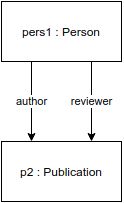
\includegraphics[width=3cm]{images/author_is_reviewer.drawio.png}
\caption{Instance model where author is also the reviewer}
\label{fig:air}
\end{figure}
% ------------------------------------------------------------------------------
% From a set theory perspective we can describe this situation as: 
% $\{h \in \Humans \mid \authors(p, h) \land \reviews(p, h)\}$.
In theory this situation can easily be detected. However, besides 
availability of the necessary data, the person executing such attack, will 
most likely not give his own name as reviewer at the moment of submitting his 
paper (it is 
normal to identify possible reviewers at submission~\cite{C2013}). The main
question here 
is, how are we able to identify the author and reviewer as the same person.

We approach this situation from a timeline perspective, which is how Moon is 
detected. A paper goes through certain stages until it is published. In
Figure~\ref{fig:timeline} we draw a timeline with the milestones of the
publication process. \textit{Submitted} is when the paper is received by the
venue. \textit{Revised} is the moment a paper is submitted again after review
with changes; the asterisks implies that this can occur multiple times, or none
at all if the paper is accepted at first submission. \textit{Accepted} defines
the state when the paper is ready for publishing. \textit{Published} is the last
step and is the date the paper is published.
Most publishers also work with an \textit{Available Online} date. Once accepted,
a paper can be placed on the website of the publisher before the journal has
been published.
% ------------------------------------------------------------------------------

\begin{figure}[H]
\centering
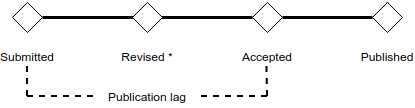
\includegraphics[width=9cm]{images/timeline.drawio.png}
\caption{Milestones in timeline publication model with publication lag}
\label{fig:timeline}
\end{figure}

The publication-lag is defined as the time between submission and acceptance.
This measure can be used as comparison with other authors within the same venue.
A low publication-lag compared with 'normal' can be used to identify interesting
cases like an abnormal short time of review. E.g. Moon was detected because the
time his work was submitted and approved by the reviewer (which was Moon
himself) was remarkable short.
% ------------------------------------------------------------------------------
\paragraph{Benign alternatives}
The possibility exists that a paper is that good, no revision is needed and the 
review did not take that much time. This also results in a low publication-lag.
% ------------------------------------------------------------------------------

\section{Implementation}
In this section we describe how we acquire the data necessary for this case
study.

The publication date is an attribute well presented in public datasets. This 
date is derivated from the publication of the venue. 
To get the dates needed to calculate the publication-lag (submitted and
accepted), we need other sources. ACM and Elsevier show the dates on their
website (as example for ACM, see Figure~\ref{fig:acm_dates}). However, these
properties are not available for all publications.

\begin{figure}[H]
\centering

\includegraphics[width=5cm]{ACM_Digital_Threats_Research_and_Practice.png}
\caption{Publication history of an article in ACM (\url{https://dl.acm.org/doi/10.1145/3442445})}
\label{fig:acm_dates}
\end{figure}

As we already used ACM in the previous case study; in this case study we
use Elsevier. Besides we already used ACM, we have proved to be able to extract
the dates from the Elsevier website in the research proposal.
When Elsevier presents an article on their website, a JSON 
document with details about the article is available in the HTML document. Among
other details, this JSON contains a date section, see 
Listing~\ref{lst:ElsevierJsonDates} (page \pageref{lst:ElsevierJsonDates}).
From a functional perspective, we need the journals of Elsevier. From these journals
we need the articles. This dependency is shown in
Figure~\ref{fig:functional_overview_elsevier}.

\begin{figure}[H]
\centering
\includegraphics[width=6cm]{images/case_study_3/implementation/functional_overview.png}
\caption{Functional overview acquisition Elsevier}
\label{fig:functional_overview_elsevier}
\end{figure}

Therefore, first step is acquisition of the journals of Elsevier.
\subsection{Journals}
Elsevier presents a list of journals they publish on their website when using
the search function. To get the journals we built a webscraper. In
Figure~\ref{fig:functional_overview_elsevier_journals} we position this tool in
the acquisition flow.

\begin{figure}[H]
\centering
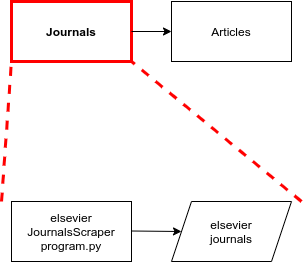
\includegraphics[width=6cm]{images/case_study_3/implementation/functional_overview_journals.png}
\caption{Acquisition of the journals}
\label{fig:functional_overview_elsevier_journals}
\end{figure}

The search functionality of Elsevier presents the journals in a paginated list
(first request returns first 100, second request 101 till 200, etc.). We can
acquire the `next results', by passing the page number as url parameter. By
using BeautifulSoup, we can parse the resulting HTML page and load required
information of the journal to the database (issn, title, href). The href is the
link to detailed information (e.g. the articles published).
The result is information of 2,970 journals. For our purpose we manually 
selected journals which we want to acquire article information here.

\subsection{Articles}
From these journals we acquire the articles. In
Figure~\ref{fig:functional_overview_elsevier_articles} we show this in the functional
landscape. We explain the details of this flow after the figure.
The first step for acquiring the article information, is downloading this 
information. We built an application for this: \verb|DownloadArticleMetadata|. 
\begin{figure}[ht]
\centering
\includegraphics[width=\textwidth]{images/case_study_3/implementation/functional_overview_articles.png}
\caption{Acquisition of the articles}
\label{fig:functional_overview_elsevier_articles}
\end{figure}

Again, we use the search functionality of the website. As search
parameters we use the name of the journal, FLA as article type (this
filters the results on research articles) and we sort by date (descending order).
The search functionality only returns 1,000 results; by using the sort function,
we acquire the 1,000 most recent articles.

The results of the search functionality are returned asynchronously. This means
the site is presented (e.g. with a loading image) while the browser sends another
request to the server to get the search results. This means that using a request
library is not possible; for this part of the solution we use Selenium
(see Section~\ref{sec:web_scraping}). The links to the articles returned in the search
results are cached. After we finished
iterating through the search results, we start acquiring the article content. This
is not asynchronous, so this is preformed with a request library.

The HTML of an article on the website of Elsevier contains an JSON part with
information about the article. In Listing~\ref{lst:ElsevierJsonDates} a part
of this JSON document is shown which contains the dates. The JSON content is
stored on disk storage for interpretation which is done by the \verb|ParseOutput|
application.

\newpage
\begin{lstlisting}[caption={Dates in the JSON document},label={lst:ElsevierJsonDates}]
"dates": {
    "Available online": "25 January 2021",
    "Received": "16 July 2020",
    "Revised": [
        "14 December 2020"
    ],
    "Accepted": "4 January 2021",
    "Publication date": "25 January 2021"
}
\end{lstlisting}

The ParseOutput application iterates through the JSON files on storage, acquires
information from these files and stores the information in the database. This
results in five tables: articles, authors, affiliations, dates and references.
As with the OpenCitations application, this tool is also multi threaded,
multiple files can be processed in parallel, to improve performance.

By using web scraping and HTML interpretation we extracted the JSON documents 
with metadata of articles across 36 journals from Elsevier (Elsevier runs 2,970 
journals). This resulted in a total of 35,136 documents. From the 35,136 we were
unable to calculate the publication-lag for 4,512 (approximately 13\%) because 
the date properties needed are missing.

% ==============================================================================
\section{Analysis and validation}
In this section we present a possible method to analyse this data. 
In Figure~\ref{fig:publication_lag_dist} we show the distribution of the
publication lag. The average is shown with a vertical red line, the median with
a black line. Every dot represents a publication.
\begin{figure}[H]
    \centering
    \includegraphics[width=\textwidth]{images/case_study_3/dist.png}
    \caption{Distribution of the publication lag (median: black, average: red.)}
    \label{fig:publication_lag_dist}
\end{figure}
Because of the right skewness in this dataset, we transpose it with $\log_{10}$ to
create a set that is more normally distributed. 
In the publications we scraped from Elsevier, we noticed 59 observations with a
publication-lag of 0 (zero). Possible explanations are:
\begin{itemize}
    \item \emph{Data quality}: It can be that this is an error on the side of
        Elsevier.
    \item \emph{Actually 0 publication-lag}: Another explanation is that the
        publication lag is actually 0. This means the article is submitted and
        accepted on the same date. 
\end{itemize}
We need to make a choice what to do with these observations because we can not
calculate the log value of a 0 publication-lag. Considering the domain we work
in it is safe to identify 0-values as outliers, because it represents a very
fast process from submission to acceptance, at least within one day. To make
sure these values are indicated as outliers, we replace $\log_{10} (0)$ with 0.
The result of this transformation is shown in
Figure~\ref{fig:publication_lag_dist_log}. We notice that the average line and
median are much closer.

\begin{figure}[ht]
    \centering
    \includegraphics[width=\textwidth]{images/case_study_3/dist_log.png}
    \caption{Distribution of the log of the publication lag.}
    \label{fig:publication_lag_dist_log}
\end{figure}

In Figure~\ref{fig:cs3_publag_iast} we plotted the log-values of every
publication-lag, ordered by author for the ACM journal Information and 
Software Technology\footnote{\url{https://dl.acm.org/journal/inst}}. 
Every dot represents a publication for one author. 
The log
of the publication-lag on the y-axis. The x-axis is an order by name of the
author (for explanation see Section~\ref{sec:cs1_analysis}).
The red dots are identified as outliers (z-score < -3, 26 days or less)
of all publications (not limited to this journal). 
The red circle in the left lower corner, we identified a 'cluster'; one author
of which the publication-lag was two times very low; 8 and 11 days (average
270, standard deviation 115).

\begin{figure}[ht]
    \centering
    \includegraphics[width=\textwidth]{images/case_study_3/publication_lag_iast.png}
    \caption{Publication lag of authors of Information and Software Technology.}
    \label{fig:cs3_publag_iast}
\end{figure}

In Figure~\ref{fig:cs3_pop_vs_poi} (page \pageref{fig:cs3_pop_vs_poi}) we 
compared the author of this cluster with the population and an authors with more 
`normal' publication-lag duration. The publication-lags of the 
person-of-interest is outlined with a red dotted box (the red striped around the 
two observations are the same as in Figure~\ref{fig:cs3_publag_iast}). In the 
green dotted-box we plotted the publication-lag times of an author which behaves 
`more' normal.
An investigation of a possible relation between the person-of-interest and any
member of the editorial board did not return notable results. The authors of
these papers were not part of the editorial board, nor did we notice an editors
of the same affiliation of one of the authors.

\begin{figure}[ht]
    \centering
    \includegraphics[width=.6\textwidth]{images/case_study_3/poi_vs_rest_vs_normal_crop.png}
    \caption{Log of the publication lag of population compared with person of interest and more `normal' author.}
    \label{fig:cs3_pop_vs_poi}
\end{figure}

\section{Case study conclusion}
In this chapter we took data of Elsevier for a a subset of journals in the
domain of Computer Science. Almost 34\% of the data we acquired from Elsevier 
was not usable for analysis. 
%
We investigated one journal and were able to identify a 
person-of-interest with two publications of which the publication-lag deviates
from other publications in the journal.

At this point we can conclude that we notice some very low, even zero, days 
between submission and acceptance of a publication. We are not able to say 
anything about the outliers. Further 
investigation can combine these properties of the publication with data of 
editors (e.g.
is the author an editor, is the editor a colleague of the author). Another
direction to investigate can be a possible pattern in reviewers and 
publication-lag. We did not found a source to get data of reviewers for a 
certain publication, but most of the times the reviewers are available at venue 
level (e.g. in the masthead).

% ==============================================================================
Considering the goal of this research; of all scraped articles of Elsevier of 
which a publication-lag could be calculated, we were able to direct the attention 
from 30,624 articles (written by 70,822 authors) to 273 articles (written by 878 
authors), if we take a threshold of 14 days. That is 0.89\% of the articles and 
1.24\% of the authors.

% ==============================================================================
\chapter{Conclusions}
\label{chp:conclusions}
% ==============================================================================

In this research we set out to direct manual investigation to notable cases.
We conclude this research with the following key findings:

% ==============================================================================
\paragraph{Lack of data quality limits creating an integrated dataset}
Source depended keys (e.g. for identifying authors) are only applicable within 
that single dataset. Therefore integrating datasets should use 
source-independent key attributes (\doi{} and \orcid{}). Ideally datasets 
containing data of the publication process should include these attributes. In 
practice the quality and availability of these source independent keys is not 
sufficient for identifying objects (see Section~\ref{sec:data_integrability}). 
This impacts the quality of the resulting integrated dataset.

Alternative approach to use names instead of \orcid{} for identifying objects
is not sufficient. However, it is possible to use alternative approaches 
(see Aminer~\cite{Tang:08KDD}); achieving a high enough level of quality 
requires a lot of effort. For the purpose of our research, we therefore conclude
that creating an integrated dataset for analysis purposes is too cumbersome.

% ==============================================================================
\paragraph{Enriching standard datasets is made more difficult because of 
diffusion coupled with lack of structure of data}
Standard available datasets are based around the author, paper, venue and 
sometimes the citation. These datasets are insufficient for generic outlier 
detection~\cite{TEJ2017}. 
%Therefore, this research aim to use a group based approach.
Standard datasets miss important data (e.g. data of PC members, 
publication-lag). In theory this data is publicly available, mostly on 
the website of publishers. In practice, this data is in an unstructured form.
Due this unstructured form, acquisition of this data and integration with
existing datasets is challenging. For example, our proof-of-concept PDF data
extractor, specifically tailored to its source material, still only achieved
a success rate of $\sim$47\% for extracting data.

% ==============================================================================
\paragraph{Applying group based approach on enriched data yields useable results}
We executed three case studies to investigate if applying a group based approach 
can indicate notable cases for manual investigation.

In the first case study we gathered the PC members from \lncs{} front matter 
documents and combined this data with \dblp{}, OpenCitations and scraped data 
from Springer Website. As an example analyses we looked at how often these 
members where cited in their own journal. For one proceeding we plotted the 
results in Figure~\ref{fig:analysis_members} (page 
\pageref{fig:analysis_members}). Depending on the threshold, we 
limited the scope for analysis from 483 member of the SPIRE proceedings to 1 
outlier.

% ==============================================================================
In the second case study we acquired the Editorial board of ACM journals. This 
data is combined with \dblp{} to get the co-authors. As a possible analysis 
method, we looked at the number of unique co-authors these editors worked with 
inside versus outside the journal. In Figure~\ref{fig:editors_in_out_journal} 
(page \pageref{fig:editors_in_out_journal}) the results of one journal are 
shown. Although not as clear as case study 1, we 
are able to direct manual investigation from 479 authors in total to 3 notable 
cases (especially observation 3 in Figure~\ref{fig:editors_in_out_journal}).

% ==============================================================================
As third case study, we focused on the time aspect of the publication process by 
looking at the publication-lag. In this case we did not integrate additional 
data. Instead of indicating the value of additional objects, we show the value 
of additional attributes for already available objects in standard datasets. We 
used data of some journals we scraped from Elsevier. In 
Figure~\ref{fig:publication_lag_dist_log} (page 
\pageref{fig:publication_lag_dist_log}) we see the deviation of the
publication-lag. On the left side we notice very low publication-lags. 
By applying a threshold of 14 days, this approach limits the subjects for 
investigation from 30,624 articles (written by 70,822 authors) to 273 articles 
(written by 878 authors).

\ \\
The question we aim to answer during this research was: \emph{To what extend 
can integration of publicly available data sources contribute to directing 
manual investigation of scientific fraud?} As answer we can formulate is that 
integrating publicly available data enables a group based outlier detection 
approach, which yields notable cases for further manual investigation.

% ==============================================================================
\paragraph{Impact of this research}
The conclusions and part of the approach of this study can result in a detection
framework that directs investigation of fraud to the most striking cases. This
improves the detection of fraud cases which eventually results in a more fair
scientific publication environment.
% ==============================================================================

\section{Future work}
We present three directions for further research: Data acquisition, Data 
integration and an alternative detection method.

\subsection{Data acquisition}
This research shows the added value of additional acquired data; PC members from 
Springer LNCS, Editors of ACM and publication-lag of Elsevier. However, these 
datasets has their weak spots which could be improved. 
In this section we propose some improvements in data and process.

\paragraph{Editorial board}
The added value of having data about the Editorial board has been mentioned 
multiple times by other researchers. In our research we used webscraping to get
the editorial board of a limited number of journals from ACM. Our approach has a 
few weak spots:
\begin{itemize}
    \item The data is limited to journals of ACM;
    \item Only the active board is acquired.
\end{itemize}
A solution that would acquire editorial board documents (comparable with the 
LNCS front matter documents) and parses these documents, would deliver high 
added value to the research in scientific fraud.

\paragraph{Review data}
Data about the review process is not publicly available. However, if we look at
the publication process, this review part has a high impact on the scientific 
performance of authors. Therefore, data about this process is valuable.
Open initiatives to review papers do exist. One of them is
Pubpeer\footnote{\url{https://pubpeer.com/}}, 
where researchers can comment on papers.
Mining this data adds value about the quality of publication process of 
venues.

\paragraph{Industrialise data acquisition}
In this research we acquired the data as a one-time effort. This results in
pieces of a possible end-to-end data pipeline (from acquisition to analysis). 
When directing for a general safety net, a more
structured approach should be set up. We propose two directions necessary for
this safety net:
\begin{enumerate}
    \item The pieces of the pipeline should be chained together to form a
        a more streamlined process;
    \item Loading complete datasets every time is cumbersome. Therefore
        acquiring deltas could improve performance of the detection process.
\end{enumerate}
% ==============================================================================

\paragraph{Front matter parsing}
From the validation of the front matter parsing proof-of-concept
(Section~\ref{sec:front_matter_parsing}, \nameref{sec:front_matter_validation}) 
it is clear that improvements are possible. This will result in a better parsing 
and therefore in more and better data.
However, this is still a quick win: only name and affiliation are available in 
these documents and formats can and will change. Our assumption is that 
continuing this approach, the amount of acquired data will not exceed the 80\% 
of available data in the front matter documents.
Therefore, the need for a machine readable standard (see recommendations) stays,
but this direction does improve the analysis on short-term; resulting data will 
certainly be better than what is available right now.

Also, besides improvement of the data acquisition tool, research could be 
conducted if the same approach and software can be applied to load documents 
from other publishers (e.g. IEEE).
% ==============================================================================

\subsection{Dataset integration}
In this research integrating multiple datasources to create one dataset was not
feasible. One reason is that people involved in the publication process were not
uniquely identifiable. Possible directions to improve the integration of people are:

\paragraph{ORCID as source}
In this research we approached integration directed from the datasources, which
may contain an \orcid{} for the author. In Figure~\ref{fig:fw_orcid_1} this is 
drawn on the left side. Another approach may be to see the \orcid{}
as source, and match people based on their publication (in \orcid{} people can 
add their publications) \textit{or} \orcid{}, shown on the right. In this new
situation, \orcid{} becomes a bridge between the sources.

\begin{figure}[H]
    \centering
    \includegraphics[width=14cm]{images/conclusions/fw_orcid_1.png}
    \caption{Left: our approach, right: proposed improvement}
    \label{fig:fw_orcid_1}
\end{figure}

\subsection{Alternative detection method}
The focus of this research is on the added value of integrating additional data 
sources. The case studies to prove this value were all executed with attacks in 
mind. Therefore, the datasets created for this analysis were focused on certain 
metrics to indicate these attacks. 
The weakness is that this approach is
still specific to each attack: for every new type of attack discovered, a new
analysis or detection method has to be implemented. 
To discover these new attacks, the community ends up relying on whistleblowers, 
which essentially brings us back to square one; no generic approach.
Our proposal is to look at the structure of the data from a graph 
representation. In Appendix~\ref{chp:graph_based_approach} we will perform an
initial exploration on this approach.

% \section{CONTINUE HEERRRREEEEE!}
% \todo{heelveel}
% voorzet, misschien generieke methode mogelijk

% generiek werkt niet op data zelf
% mss wel op graaf representatie, in volgende hfst

% nu nog steeds kijken welke outliers we geintreseerd zijn
% tielenburg? misschien outcount niet goed genoeg

% voorstel kijken naar cycle


% ==============================================================================
\section{Recommendations}
\label{sec:recommendations}


The most recommendations we present are for the publisher.

\paragraph{Machine readable standard}
As we shown in this research, currently valuable data is available, but:
\begin{itemize}
    \item In an unstructured manner (some in PDF documents, e.g. editors, some 
        data on website e.g. dates);
    \item Every publisher provides this data differently.
\end{itemize}
This results in problems acquiring this data:
\begin{itemize}
    \item Lots of publisher-fitted procedures should be implemented;
    \item It is not possible to separate between data not known, or data not 
    presented.
\end{itemize}
% ==============================================================================
This last point is important. Consider the following two structures to represent
a person. In Listing~\ref{lst:rec_ex_not_known} (page
\pageref{lst:rec_ex_not_known}) the ORCID element is 
provided, but it is not known. The receiver (client requesting this data) knows 
that the ORCID is not known by the sender (which is eventually also information 
about data-completeness). In 
Listing~\ref{lst:rec_ex_not_present}, it is unknown if the sender knowns the 
ORCID, but is not presenting it, or if the sender don't know the ORCID, and 
therefore not sending this value.
Therefore, our recommendation is to define a machine-readable standard for data 
exchange with no optional fields (values can be null).
With a standard in place, more research based on improved data can be conducted,
which eventually leads to more fraud detected.


\begin{figure}[!h]
    \begin{minipage}{0.5\textwidth}
        \begin{lstlisting}[
            caption={Example of not known data},
            captionpos=b,
            label={lst:rec_ex_not_known}
        ]
        "Person": {
            "FirstName": "Jodocus",
            "LastName": "Kwak",
            "ORCID": null
        }
        \end{lstlisting}
    \end{minipage}
    \begin{minipage}{0.5\textwidth}
        \vspace{15pt}
        \begin{lstlisting}[
            caption={Example of not presented data},
            captionpos=b,
            label={lst:rec_ex_not_present}
        ]
        "Person": {
            "FirstName": "Jodocus",
            "LastName": "Kwak"
        }
        \end{lstlisting}
    \end{minipage}
\end{figure}


% ==============================================================================
\paragraph{Apply fraud detection on the process}
Currently automatic fraud detection procedures are in place for publication 
content, e.g. plagiarism. On the publication process side, most publishers have 
a code of conduct. However, we are unaware if automatic detection of fraudulent 
behavior is in place.
% ==============================================================================
Therefore, our recommendation is to:
\begin{itemize}
    \item Make detection of fraudulent behavior an integral part of the 
        publication process;
    \item If procedures are in place, provide information to the public that the 
        publication process is being monitored for fraudulent behavior.
\end{itemize}
The result is that people with malicious intent become restrained in attacking
the publication process.

% ==============================================================================
\paragraph{Make more data about the review process public}
Data about the review process is not publicly available. However, this review 
process is essential for the scientific community; this is the
`self-controlling’ element that leads to a certain research quality.
This is also a weak spot; the result of the review entirely depends on the 
reviewer, which may, or may not, be personally involved.
Therefore our recommendation is to provide metadata about the review process, 
e.g:
\begin{itemize}
    \item Who reviewed which paper;
    \item When was the paper presented to the reviewer;
    \item When was the result of the review returned;
    \item What was the result;
    \item What methodology was applied (e.g. single-blind, double-blind).
\end{itemize}

Providing this data to the community will result in monitoring the review 
process on personal involvement and therefore forces the review to become 
more about the research instead of the researcher.

% ==============================================================================
\paragraph{ORCID}
During analysis of the scraped data from Springer, we ran into cases where an 
author has multiple ORCID's. Checking these ORCID's at \url{https://orcid.org/} 
made clear that these are indeed the same person, but working at different 
universities.
Our recommendation for researchers therefore is to use one ORCID consistently.

% \paragraph{Make more data available}
% For publishers it is little effort to make more data available. As example, the
% dates of the publication process to get the publication-lag is available for
% publishers and is a major enrichment of existing datasets.

% \paragraph{Make data machine-readable}
% It would be a major improvement if publishers make data of editors and PC
% members machine readable available. As of now, the documents (front matter,
% editorial notes) containing these people do not include the ORCID. This makes,
% sense, the document is meant for humans, but for data integration and analysis
% purposes, this would be a big improvement.

% \paragraph{Improve (and measure) data quality}
% One conclusion is that due to lack of data, we were unable to create an
% integrated dataset. The two attributes to start with should be the ORCID and
% DOI. Detection should be in place to detect if a person has multiple ORCID's,
% or none. A sanity check can be put in place if the ORCID delivered by the author
% is correct by cross-referencing \url{https://orcid.org/}.

% \paragraph{Stick to one ORCID}
% During analysis of the scraped data from Springer, we ran into cases where
% an author has multiple ORCID's. Checking these ORCID's at
% \url{https://orcid.org/} made clear that these are indeed the same person, but
% working at different universities. Therefore, for authors; please stick to one ORCID.

% \paragraph{Apply more fraud detection by publishers}
% \label{p:recom:fraud_detection_publishers}
% Due incorporate quality assurance in the publication process and propagate this
% to the community, the value of publishing at a venue of this publisher may
% increase, which is beneficial for all venues of the publisher.
% If the value increases, other publishers will be forced to also take action
% which results in less fraud altogether.

% ==============================================================================
\section{Discussion}
\label{sec:discussion}

% \paragraph{Automatic detection of fraud in the publication process}
% Because the publication process always involves human interaction, we should 
% always ask for explanation when curious behaviour is detected.


In this research we found that applying group based outlier detection on 
enriched datasets with publicly available data 
can direct manual investigation to notable cases. This means that 
valuable data is `hidden’ in PDF documents and shown on websites. 

The fact that we can detect outliers does not mean that we can detect fraud, we
can only address outliers. As stated in the introduction, the underlying
assumption of this research is that fraudulent behavior will be reflected as
outliers, but not all outliers are fraud. This raises the question raises if we
will ever be able to set up a system that detects fraud in the scientific
publication process. In our opinion, we should always apply for fair hearing.


Our main goal was to propose an approach to direct manual investigation to 
notable cases. Theoretically, this approach can be applied for that goal. 
However, we are unable to determine if this actually results in finding frauds. 
A more comprehensive study with current ‘catches’ compared with investigation of 
outliers found by our proposed approach should provide the conclusion if this 
approach pays off.

We can not state that we find an enormous number of interesting cases; this 
depends on the threshold that defines the outlier. However, the threshold we 
put in place during the case studies were high. Investigating the list of 
outliers from most to least, will eventually reach a point that investigating 
does not pay off anymore. The border before that moment can be set as a 
threshold. Only then we know how successful our approach is in actually 
finding frauds.




% ==============================================================================

\paragraph{Addressing cross-publisher fraud}
% ------------------
Current fraud detection mechanisms typically focus on the content of the 
publication. However, as argued in this thesis, data on the publication process 
may be leveraged to uncover forms of fraud that have escaped notice so far. One 
example of such a fraud is `lightweight' fraud that is repeated across many 
publishers. This fraud becomes impactful due to the quantity of affected works, 
not the impact of a single fraudulently published work.
Addressing such fraud requires at the very least integration of data from 
different publishers.

A solution could be an independent institute which receives the necessary data 
to do cross-publisher analysis. This institute could serve as a provider for
analytical services for publishers unable to set up this necessity themselves.
The responsibility of this institute is to address and investigate notable 
cases. Funds for such an institute may come from institutes that gain from a fair
publication-process. In the Netherlands this may be the NWO (Dutch Organisation
for Scientific Research), or a partnership of universities.

% ==============================================================================

%     \begin{itemize}
%         \item Op generieke manier wetenschappelijk fraude detecteren, kan dit automatisch?
%         \item Misschien meer data
%         \item Imago schade als publishers niet meewerken
%     \end{itemize}
% One way to decrease fraud in the publication process is to step away from the
% current way of judging a researcher. The University of Utrecht is moving to 
% another method to judge their researchers based on their effort to promote open
% research and their teamwork 
% \footnote{\url{https://www.nature.com/articles/d41586-021-01759-5}}. With this 
% movement the university is abandoning the indices based on publications and 
% citations.
% \begin{itemize}
%     \item Hoe kan men dan oordelen waar budget heen moet?
%     \item Hoe beoordeelt men de toegevoegde waarde van een onderzoeker 
%     objectief?
%     \item Wat is de impact hier van op de 'piramide'-structuur van 
%     universiteiten?
%     \item Hoe kunnen medewerkers bij de UU de overstap maken naar een 
%     universiteit die beoordelingen wel basseren op impact factor?
    
% \end{itemize}





% \outline {
% \paragraph{meer data openbaar maken}
% \begin{itemize}
%     \item bijvoorbeeld publicatielag
%     \item Niet spannend (weinig moeite voor publishers), wel grote verrijking
% \end{itemize}
% \paragraph{Meer fraud detectie inzetten door publishers}
% \begin{itemize}
%     \item Kwaliteit van dit stukje van het publicatieprocess borgen.
% \end{itemize}
% }



% \outline{
% \begin{itemize}
%     \item Samenvatten
%     \item Niet alleen samenvatting!
%     \item Wat is de impact op de wereld? Wereldvrede :)
%     \item Wat zouden we moeten doen en hoe kunnen hiervan profiteren?
%     \item Misschien combineren met Discussions?
%     \item Voorbeeld discussions
%     \begin{itemize}
%         \item Op generieke manier wetenschappelijk fraude detecteren, kan dit automatisch?
%         \item Misschien meer data
%         \item Imago schade als publishers niet meewerken
%     \end{itemize}
%     \item Misschien combineren met recommendations
%     \begin{itemize}
%         \item Informatie machine-readable aanleveren
%     \end{itemize}
%     scientific repeat.
% Conclusions repeat the key findings... *and* their impact. Typically, the impact is more important than the main findings. For example, "we found 37 sites out of 50 were vulnerable" is what you did. To that, you add what this means: how worrisome is this? what should be done now that we know this? How can we improve the world?
% \end{itemize}



% \section{Discussion}

% }



% % ==============================================================================
% \chapter{Recommendations}
% \label{chp:recommendations}
% % ==============================================================================
% \outline {
% \paragraph{meer data openbaar maken}
% \begin{itemize}
%     \item bijvoorbeeld publicatielag
%     \item Niet spannend (weinig moeite voor publishers), wel grote verrijking
% \end{itemize}
% \paragraph{Meer fraud detectie inzetten door publishers}
% \begin{itemize}
%     \item Kwaliteit van dit stukje van het publicatieprocess borgen.
% \end{itemize}
% }

% ==============================================================================

%%\backmatter

\newpage


\pagenumbering{roman}

\bibliographystyle{alpha}
\bibliography{report}


%% update look of titles
\titleformat{\chapter}[display]{\bfseries\filcenter}{\huge\appendixname~\thechapter}{2ex}{\LARGE}

%% Use letters for the chapter numbers of the appendices.
\appendix

\begin{landscape}

\chapter{Dataset PC Member citations}
\label{appendix:dataset_pcmember_citation}

% \begin{multicols}{2}
% \begin{wrapfigure}{r}{0.75\textwidth}
%     \centering
%     \includegraphics[
%     % height=19cm,
%     width=\textwidth,
%     angle=90
%     ]{images/dag_lncs_members_citations.png}
%     \caption{Dataset composition PC Member citations}
%     \label{fig:dataset_pc_member_citation}
% \end{wrapfigure}
\begin{figure}[H]
    \centering
    \includegraphics[
        % angle=90, 
        width=25cm,
        % height=19cm
        ]{images/dag_lncs_members_citations.png}
    \caption{Dataset composition PC Member citations}
    \label{fig:dataset_pc_member_citation}
\end{figure}

\begin{itemize}
    \item \emph{Green nodes}: Source tables, tables loaded by acquisition
        tooling.
    \item \emph{Blue nodes}: Tables or views.
    \item \emph{Lan prefix}: Tables with attributes in correct format and indexed
        for performance.
    \item \emph{Stg prefix}: Tables ready for integration. More `business like'
        objects (e.g. Person, Article).
\end{itemize}
% \vspace{\fill}
% \begin{description}
%     \item[Green nodes] Source tables, tables loaded by acquisition tooling.
%     \item[Blue nodes] Tables or views.
%     \item[Lan prefix] Tables with attributes in correct format and indexed for performance.
%     \item[Stg prefix] Tables ready for integration. More `business like' objects (e.g. Person, Article).
% \end{description}
% \end{multicols}



\end{landscape}



\chapter{Research Proposal: Exploration of abstract graph-based approach to outlier identification}
\label{chp:graph_based_approach}
% ==============================================================================

This proposal is to find a common denominator across attacks by approaching the 
publication process domain from a graph perspective.

Figure~\ref{fig:graph_1} shows a graph representation of self-citation.
Note that this is a 3-cycle directed graph: a person (node) authors (edge) a 
paper (node) which cites (edge) a paper (node) written by the same author (the 
first node).

\begin{figure}[H]
    \centering
    \includegraphics[width=8cm]{images/conclusions/future_work_graph/1.png}
    \caption{Graph representation of self-citation}
    \label{fig:graph_1}
\end{figure}

For readability we flatten this graph in Figure~\ref{fig:graph_2}. These are 
exactly the same situations. Person A on the left is the same as Person A on
the right (dotted line); in this chapter this notation is used to represent
the same node.

\begin{figure}[H]
    \centering
    \includegraphics[width=8cm]{images/conclusions/future_work_graph/2.png}
    \caption{Graph representation of self-citation, flatten}
    \label{fig:graph_2}
\end{figure}

If a person `attacks' the publication process by an exorbitant number of 
self-citations, this graph would extend as in Figure~\ref{fig:graph_3}.

\begin{figure}[H]
    \centering
    \includegraphics[width=8cm]{images/conclusions/future_work_graph/3.png}
    \caption{Graph representation of multiple self-citations.}
    \label{fig:graph_3}
\end{figure}

As such, the representation of a person that publishes in the venue he is editor
of, is shown in Figure~\ref{fig:graph_4}. This situation can be extended as in
we did in Figure~\ref{fig:graph_3}.

\begin{figure}[H]
    \centering
    \includegraphics[width=8cm]{images/conclusions/future_work_graph/4.png}
    \caption{Graph representation of publishing in own journal.}
    \label{fig:graph_4}
\end{figure}

\newcommand{\ewcount}{\mi{count}}

In this research, an outlier is defined a an observation which matches or 
exceeds a thresholds; we define what is considered normal behaviour and 
indicate outliers. Now lets consider the following situation:
\[ \text{Let}\ A1=\text{self-citation attack (Figure~\ref{fig:graph_2})}. \] 
\[ \text{Let}\ A2=\text{self-publishing attack (Figure~\ref{fig:graph_3})}. \] 
\[ \text{Let}\ x=\text{outlier threshold set to 3}. \]
\[ \text{Let}\ \ewcount(A1)=2. \]
\[ \text{Let}\ \ewcount(A2)=2. \]

If we apply detection mechanisms as described in this research, both attacks 
are not considered an outlier (because $2 < 3$).
However, for the person applying these attacks, the total of `gains' he has
is 4 ($\ewcount(A1) + \ewcount(A2)$). Attackers who take these thresholds in 
account (and therefore stay under the radar), will not be detected. This 
situation is represented in Figure~\ref{fig:graph_5}.

\begin{figure}[H]
    \centering
    \includegraphics[width=11cm]{images/conclusions/future_work_graph/5.png}
    \caption{Two types of attacks.}
    \label{fig:graph_5}
\end{figure}

We see 4 paths, 2 for every attack; so considering the threshold $x$, this 
should be an outlier. 

A person will attack the publication process to improve its own metrics.
Therefore, the assumption that this future work proposal is based upon, is
that an attack can be considered a path from and to the 
same person.
An abstraction of this fraud detection approach is shown in 
Figure~\ref{fig:graph_7}; an attacker as Node A which performs $N$
attacks, visualized by the paths $1$ till $N$.

\begin{figure}[H]
    \centering
    \includegraphics[width=8cm]{images/conclusions/future_work_graph/7.png}
    \caption{Abstraction of paths.}
    \label{fig:graph_7}
\end{figure}

\newcommand{\incoming}{\mi{incoming}}
\newcommand{\outgoing}{\mi{outgoing}}
\newcommand{\isperson}{\mi{isperson}}
\newcommand{\isaffiliation}{\mi{isaffiliation}}
\newcommand{\isjournal}{\mi{isjournal}}

Considering this abstraction. We can set the following:
\[ \text{Let}\ n=\text{Node}. \] 
\[ \text{Let}\ p=\text{Path}. \]
\[ \text{Let}\ \isperson(n)=n\text{ is of type person.} \]
\[ \text{Let}\ \outgoing(n, p)=\text{path }p\text{ is outgoing of node }n\text{.} \]
\[ \text{Let}\ \incoming(n, p)=\text{path }p\text{ is incoming in to node }n\text{.} \]

The count of collection of paths of a person which eventually returns to 
the same person can than be expressed with Predicate~\ref{eqn:path_count}.
\begin{equation}
\label{eqn:path_count}
\forall n (\isperson(n) \implies \forall p(\outgoing(n, p) \land \incoming(n, p)))
%%\caption{Counting paths.}
\end{equation}


\paragraph{Benefits}
This approach has the following benefits:
\begin{itemize}
    \item At forehand specified derived metrics are not necessary (e.g. 
        \textit{count of citations} or \textit{count of publications}), the only 
        interesting metric becomes the \textit{count of paths}.
    \item \textit{How} the publication process is being played becomes less 
        relevant for detection. This approach indicates \textit{that} the 
        process is being played. Although this should not neglect the analysis
        of the attack to gain knowledge of attacks.
    \item Changing the \isperson() to \isjournal() or even \isaffiliation(),
        abstracts the type of the attacker. With this approach 
        attacks of journals to improve their Journal Impact Score or 
        affiliations that behaves like a high performing research facilities can
        be investigated.
\end{itemize}

\paragraph{Caveats}
This approach comes with some caveats:
That fact we reason about a directed graph is important. Also, the 
roles of the edges should not taken lightly. For example: If a person
\textit{authors} an article, the article is \textit{written by} that person 
(Figure~\ref{fig:graph_8}). Theoretically, this results in a cycle which will be 
counted in Predicate~\ref{eqn:path_count}.
  
\begin{figure}[H]
    \centering
    \includegraphics[width=5cm]{images/conclusions/future_work_graph/8.png}
    \caption{2-Path cycle to neglect.}
    \label{fig:graph_8}
\end{figure}

To prevent this, some measures should be taken. E.g.:
\begin{itemize}
    \item Set a minimum count of edges (e.g. neglect paths with less than 3 edges);
    \item Set a guard on the label of edges that inputs and outputs an attack.
\end{itemize}
% % ==============================================================================


% \input{Appendices/appendix-a}
%  \input{Appendices/appendix-b}
%  \input{Appendices/appendix-c}


% \chapter{VANAF HIER ONZIN}

% % ==============================================================================
% \section{General process}
% Bjorn and hedlund descirbed the publication process from a cost perspective 
% \cite{BH2004}. We can use this to visualize the publication process from a time 
% perspective. This view is input to determine if we are able to collect all 
% necessary metrics.



% % ==============================================================================
% \section{Flow proceedings and conferences}


% % ==============================================================================
% \subsection{Group identification}
% % ==============================================================================
% The first step in detecting outliers is to identify groups of people who are in 
% the same position. We identify the followig groups in his research because they
% may be interesting.

% \paragraph{Editors of proceedings}

% \paragraph{Authors submitting at the same conference}

% \paragraph{Author submitting at the same journal}

% \paragraph{Authors that publish with each other}

% \paragraph{H-Index}



% % ==============================================================================
% \chapter{Data integration}
% % ==============================================================================

% \section{References}







% \section{Integration}
% People, articles and venues are retrieved
% from multiple source. To be able to work with these entities, we need to 
% integrate these sources in one model. To make this possible, we need to 
% unqiquely identify the entities.

% Again refering to Figure~\ref{fig:dataflow_jm2017}, we can consider this the 
% tilde sign.

% In the ideal situation al entities have an unique identifier which is 
% independent of the source. However, in practice it is a bit more complex than 
% that.



% \subsection{Articles}
% For all chapters from Springer LNCS we scraped the unique document identifier 
% (DOI). DOI should be unique of all documents.

% However, an analysis of the DBLP data set leaves us with a few DOI's which refer
% to mutliple articles. The number of articles this occurs, is very low.

% DBLP also has a lot of documents where the DOI is unknown; so data completeness 
% is an issue here. 

% For references we use opencitations. Because opencitations is DOI based, it is 
% very good integreerbaar with LNCS.

% % === oud, weg misschien
% % However, this document id is not filled in for all titles. For
% % the papers that do not have an doi, we can do the match on title. Unfortunately,
% % this also is not that straightforward. The title sometimes contains latex 
% % specific characters, or other weird characters.


% \subsection{Uniquify people}
% The author dataset contains all authors for every article. This means, if an 
% author wrote multiple articles, it is multiple times present in this set. For
% our use case, this is not sufficient; we need identify these people as the same 
% person, otherwise collecting metrics for a person is impossible.

% The set we achieved from LNCS conains name, orcid and email. An analysis of this
% set made clear that we got the same name with multiple orcid, or one orcid that 
% refers to more than one person. Concluding: a name does not make a person 
% unique.

% Luckely, DBLP acknowledges this problem. Although they do not yet have all 
% authors unique, they are working on this problem and provide a way to get the 
% unique persons already identified.

% DBLP has the relation between author and article, so to get the `correct' author
% of an article, we need to match the articles in DBLP with the chapters in LNCS.


% % \subsection{Article integration}
% % Not only do we need to match the articles of DBLP and Springer LNCS, we also 
% % need to incorporate Aminer. Aminer is an enrichment of DBLP in that it adds
% % citations. Although DBLP is working to incorporate citations in their dataset,
% % this is still work in progress and Aminer has already a lot of that data.

% % \begin{figure}[H]
% %     \centering
% %     \includegraphics[width=10cm]{images/linking_article_dblp_lncs_aminer.drawio.png}
% %     \caption{Matching Springer LNCS, DBLP and Aminer}
% %     \label{fig:linking_article_dblp_lncs_aminer}
% % \end{figure}



% \section{Nog onbenoemd}


% To get an integrated dataset across all sources some challenges need to be 
% addressed. Also, to be able to integrate the sources where we need to get the
% data from, we sometimes need to get data from another source.

% The main entities we need to integrate are person (authors, members of program
% committees etc.) and articles (chapters from lncs with papers from aminers).

% \section{Integration of persons}

% First challenge is to make the authors unique. This comes with the
% second challenge of data quality.

% For example, from springer we scrape get the chapters (inproceedings) and their 
% authors from their site. This authors sometimes comes with an orcid, which 
% should be unique. However, we found situations where an author gets an orcid of
% someone else. This is a data quality issue.

% Luckely, this does not occur much, and for the few it occurs we can easily 
% create a manual file to override this. Of course with caution; if two orcid 
% have the same name, we can not override this; some authors have the same name.
% On the other hand, if one orcid refers to a totally different name, we can.


% Seconds challenge is that a name does not make an author unique. The same name
% refers to other authors. Luckely, DBLP addresses this problem by suffixing the
% name with a four digit code~\footnote{\url{https://dblp.org/faq/1474704.html}}.
% DBLP is making progress here, but this is not entirely done yet. But even if
% they mention to unique identity authors, the match to authors in other 
% datasources (like Aminer and Springer) is not straightforward. In that case we 
% need to ignore the authors from these sources and make the match by going 
% through the paper (or chapter, as is it is called within LNCS Springer).

% Third challenge is the name. For most authors these sources do not contain an
% orcid or an email address, which means we need to match the authors on name.
% But, in some sources the names are fully written (with or without the 
% middlename), sometimes the middlename only has a initial while the firstname is 
% fully written, and sometimes we only get the initials and lastname.
% DBLP covers this by naming all aliases of a single person.

% Still we do have a problem, because inthe end we need to match these authors
% with members we get from the frontmatters of lncs. Within this frontmatters, 
% there is no orcid, email, or a four digit number to match to dblp records; these
% documents or not written with the intention to identify persons.

% \subsection{Approach}
% \begin{itemize}
%     \item Get DBLP data dump and create unique authors. DBLP also has their 
%         aliases and sometimes orcid.
%     \item Also use this dump to get the inproceedings, incollections and 
%         articles.
%     \item This dump can also be used to create the author relationship between 
%         articles and persons.
%     \item Integrate springer lncs chapters into the article entity.
%     \item Use springer lncs to get the book (collection) and identify the 
%         relationship between chapter and book.
%     \item Integrate members from the frontmatter into the person entity.
%     \item Use he frontmatter to lay the relationship between the proceeding and
%         the person.
%     \item *** Now we can get a few groups
%     \item Integrate the aminer papers in the article entity.
%     \item Use aminer to get the relationship between articles.
% \end{itemize}


% % ==============================================================================
% \chapter{Data integration}
% % ==============================================================================
% \outline{
%     \begin{itemize}
%         \item Three main sets to intergrate: Humans, Venues, Publications
%     \end{itemize}
%     \section{Publication}
%     \begin{itemize}
%         \item Root is DBLP
%         \item Key is DBLP key
%         \item We need to integrate the publications from DBLP with Aminer
%         \item DBLP is leading, so we need to match publications from dblp to aminer
%         \item In two steps: First try to match on DOI, second, match on title
%     \end{itemize}
%     \subsection{Document Object Identifier}
%     \begin{itemize}
%         \item Wat is het? DOI is unique identifier of a document
%         \item 
%     \end{itemize} 
%     \subsection{Enrichtment of DOI's}
%     Some publication do not have an DOI in DBLP, but provide an additional link to arxiv site, or wikidata
%     \paragraph{Arxiv}
%     \begin{itemize}
%         \item Arxiv sometimes has a DOI (but not always).
%         \item We extact docuemnt information from the Arxiv API. As we were there, we also extracted the authors.
%     \end{itemize}
%     \paragraph{Wikidata}
% }



% \outline{
% \begin{itemize}
%     \item Onderzoeksvraag: Welke data is nodig en hoe kom je eraan?
%     \item Doelstellingen:
%     \begin{itemize}
%         \item Data verzamelen
%         \item Data analyseren
%     \end{itemize}
% \end{itemize}
% }




% % ==============================================================================
% \chapter{Data Acquisition}
% % ==============================================================================
% \outline{


% \outline{


% }

% \section{Our root: Computing Research and Education Association of Australasia ranking}
% \begin{itemize}
%     \item CORE
%     \item Australian based, so might be biased
%     \item A website which ranks conferences and journals
%     \item Ranking is from A* to C. Our focus is for the ranking A*, A and B
%     \item The conference list contains the following attributes:
%     \begin{itemize}
%         \item Title
%         \item Acronym
%         \item Rank
%         \item DBLP link
%     \end{itemize}
% \end{itemize}
% \subsection{Gathering the data}
% \begin{itemize}
%     \item Choices for data acquisition:
%     \begin{itemize}
%         \item Use the export functionality on the website
%         \item Scrape the data from the HTML pages
%     \end{itemize}
%     \subsection{Methods}
%     \paragraph{Export functionality}
%     The core websites offers the functionality to download all the data in a CSV file. This is very useful, because 1) this allows us to get the data in a format that is simple to process in a database (we can consider this a table) and 2) it is fast to get the data.
    
%     The drawback however is that this data does not contain the DBLP url. This means we are not able to find related data in a structured manner.
%     A possible way to work with this problem is to manually add the dblp url's ourselves, but this is a labour intensive job, comes with a cost in reproducability and, because of the manual effort, is error-prone.
    
%     \paragraph{Webscraping}
%     \begin{itemize}
%         \item The core website contains the data in a HTML table accross multiple pages.
%         \item With GET request able to get this -> so we are able to automate this.
%         \item All data that is in the table is at our disposal.
%         \item Also the dblp url in the href of the Anchor tag.
%         \item Drawback: Need to build a script for it, which take more time than simply click the export button.
%     \end{itemize}
    
%     \paragraph{Copy-pasting from the website}
%     \begin{itemize}
%         \item Html table, so easy to paste in a table
%         \item Manual work: not convenient for reproducability
%         \item Also unable to find the DBLP url (we only get the 'view'-text in this case)
%     \end{itemize}
    
%     \paragraph{Method conclusion}
%     \begin{itemize}
%         \item We choose to build a script to scrape the data over downloading the export
%         \item Main reason was reproducability and less error prone in finding the DBLP urls.
%     \end{itemize}
    
%     \subsection{Process}
%     \begin{itemize}
%         \item pagination is given in the url
%         \item While testing the site we discovered that when requesting a page outside the pagination number, we did not get a 200 (OK) response
%         \item Loop through pages untill we do not get a 200 (OK) response
%         \item Get the data from the table
%         \item Write it to database
%         \item build in python because... not really a reason except it's hip and happening (and I honestly don't know why)
        
%     \end{itemize}
    
%     \subsection{Result}
%     \item The result was the data presented in two tables in schema 'core': 1) conf-ranks (conference rankings) and jnl-ranks (journal rankings)
%     \paragraph{Completeness}
%     Core conference data:
%     \begin{itemize}
%         \item 883 rows in total, within scope (because of rank): 486
%         \item No DBLP link for 24 conferences within our ranking focus.
%         \item To get this data we manually looked up the dblp url and added this data to the database. We were able to to find the dblp urls of 17 conferences, which remains 7 unknown
%     \end{itemize}
    
    
%     \item From this point we split the data acquisition process in two lanes:
%     \begin{itemize}
%         \item Conference tracks
%         \item Journal tracks
%     \end{itemize}
    
    
% \end{itemize}


% \section{Conference track}
% \begin{itemize}
%     \item Input is conf-ranks form core combined with manual searched DBLP urls
%     \item Purpose is to get the proceedings of the conferences
%     \item One conferences has one or more proceedings
%     \item DBLP contains this data
% \end{itemize}

% \subsection{Gathering DBLP data}
% \paragraph{Methods}
% \begin{itemize}
%     \item Download DBLP database
%     \begin{itemize}
%         \item Already done in project preparation
%         \item BUT; looking for certain proceedings were not available in download, but do on web
%     \end{itemize}
%     \item Use the API
%     \begin{itemize}
%         \item DBLP offers an API to download information.
%     \end{itemize}
% \end{itemize}
% We used the API to extract the data. Because the data is more complete.

% For all conferences in the core table (combined with some manual adjustment), we extracted the proceedings from DBLP.
% This resulted in 15994 proceedings.

% Looking for the most used publisers:
% \begin{table}[h]
% \begin{tabular}{ll}
% \hline
% Publisher & \# of proceedings \\ \hline
% Springer  & 4674              \\
% ACM       & 4010              \\
% IEEE *    & 3592             
% \end{tabular}
% \end{table}
% *IEEE also includes IEEE Computer Society
% } % END OUTLINE

% \section{PDF Reading}
% \outline{
% \begin{itemize}
%     \item Uitdiepen complexheid PDF extractie
% \end{itemize}
% }
% \begin{itemize}
%     \item PDF is mostly text plotted on a sheet with certain coordinates and properties. (also images, but we are not interested in these)
%     \item options: PDF to html
%     \begin{itemize}
%         \item Problem changed from interpreting PDF to interpreting HTML
%         \item Still need to be able to 'understand' the relationships between certain elements on the page
%     \end{itemize}
%     \item OCR (tesseract)
%     \begin{itemize}
%         \item OCR is a technology to detect characters from images
%         \item PDF is not an image, so first need to convert the PDF's to images
%         \item Output is plain text or TSV. Lot of contect (like position) gets lost in the process. This information is crucial if we want to interpret the pages.
%     \end{itemize}
% \end{itemize}
% \subsection{pdf to html}
% \begin{itemize}
%     \item Volgende libraries geprobeerd:
%     \begin{itemize}
%         \item PDFMiner
%         \begin{itemize}
%             \item Tries to split blocks of text
%             \item can be nice, but in these kind of documents, there is mostly a relation between the columne (like 'person' and an 'affiliation')
%         \end{itemize}
%         \item pdf2htmlex
%         \begin{itemize}
%             \item Most promising
%             \item Lots of CSS
%             \item Spaces can be tricky. Sometimes there is a space, but with a margin class with a negative number, so letter-space minus the margin, becomes so little, we have to ignore this space.
%             \item on the other hand, sometimes there is no space, but the space needs to be derived from the letter-spacing.
%             \item other challenge are items in a column that do not fit the row, so it continues on the next row. How do we consider this text as part of which column?
%         \end{itemize}
%     \end{itemize}
% \end{itemize}
% \subsection{Interpreting HTML}
% \begin{itemize}
%     \item what is the scope of the document we need? For LNCS, Springer provides a template where this section is calles 'Organization'. This is not used in all cases. From whcih point in time did they choose to use this template? Are there other keywords we can use? (like of a lot of subsection headers contain words like 'committee' or 'chair').
%     \item Can we set the scope by interpreting the format? Most of the lists with names are columns.
%     \item When do we consider an element an affiliation? it seems that most (if not all) affiliation have a comma to wplit the country name.
%     \item Can we consider all elements in a column if most of them have a comma as affiliation? No, sometimes names are also <lastname>, <firstname>. But when this is the case, this happens at the first column also, and affiliatons are not likely to be placed in the first column.
% \end{itemize}
% Approach 1: Directly raed HTML elements and see if we can make this work for the LNCS frontmatters.
% \begin{itemize}
%     \item Not sustainable
%     \item hard to maintain
%     \item lots of if-then rules
%     \item good first step to see what is working and what we need to take into account
% \end{itemize}
% Approach 2: First create a model of the HTML document, from this model create a graph with sectionheaders and sections.
% \begin{itemize}
%     \item How to detect section headers? Option; get the font-size that is most used. consider this as the size of the content. Everything that is bigger, assume headers.
% \end{itemize}





\end{document}
